% ============================================================================
%  GeoEq Handbook -- A complete reference book for the geoeq Python library.
%
%  Compile with:   latexmk -pdf GeoEq-Handbook.tex
%  Or:             pdflatex GeoEq-Handbook && makeindex GeoEq-Handbook
%                  && pdflatex GeoEq-Handbook && pdflatex GeoEq-Handbook
% ============================================================================
\documentclass[11pt,a4paper,openany]{book}

% ----- Packages -------------------------------------------------------------
\usepackage[utf8]{inputenc}
\usepackage[T1]{fontenc}
\usepackage{lmodern}
\usepackage{microtype}
\usepackage[margin=1in,headheight=14pt]{geometry}
\usepackage{amsmath,amssymb,amsthm,mathtools}
\usepackage{siunitx}
\usepackage{graphicx}
\usepackage{xcolor}
\usepackage{tcolorbox}
\tcbuselibrary{breakable,skins,listings}
\usepackage{listings}
\usepackage{tabularx,booktabs,array,longtable}
\usepackage{hyperref}
\usepackage{enumitem}
\usepackage{titlesec}
\usepackage{fancyhdr}
\usepackage{makeidx}
\usepackage{epigraph}

\hypersetup{
  colorlinks=true,
  linkcolor={blue!60!black},
  urlcolor={blue!60!black},
  citecolor={blue!60!black},
  pdftitle={GeoEq Handbook},
  pdfauthor={Ripon Chandra Malo}
}

% ----- Branding colors ------------------------------------------------------
\definecolor{geoBlue}{HTML}{1E4D8F}
\definecolor{geoNavy}{HTML}{0C1A3A}
\definecolor{geoLight}{HTML}{DBEAF7}
\definecolor{geoAccent}{HTML}{E8A825}
\definecolor{geoMono}{HTML}{F8F9FB}
\definecolor{geoGreen}{HTML}{27AE60}
\definecolor{geoRed}{HTML}{C0392B}

% ----- Listings -------------------------------------------------------------
\lstdefinestyle{pythoncode}{
  language=Python,
  basicstyle=\ttfamily\footnotesize,
  keywordstyle=\color{geoBlue}\bfseries,
  commentstyle=\color{gray}\itshape,
  stringstyle=\color{geoAccent!80!black},
  numberstyle=\tiny\color{gray},
  numbers=left,
  numbersep=8pt,
  backgroundcolor=\color{geoMono},
  frame=single,
  rulecolor=\color{gray!30},
  framesep=4pt,
  breaklines=true,
  showstringspaces=false,
  literate={->}{{$\to$}}{1}
}
\lstdefinestyle{output}{
  basicstyle=\ttfamily\footnotesize\color{black!75},
  backgroundcolor=\color{white},
  frame=leftline,
  rulecolor=\color{geoAccent},
  framesep=4pt,
  breaklines=true,
}
\lstset{style=pythoncode}

% ----- tcolorbox styles -----------------------------------------------------
\newtcolorbox{funcbox}[1]{
  enhanced, breakable,
  colback=geoLight!30, colframe=geoBlue,
  fonttitle=\bfseries\ttfamily,
  title=#1,
  arc=2pt, boxrule=0.8pt,
  left=8pt, right=8pt, top=6pt, bottom=6pt,
  attach boxed title to top left={xshift=8pt, yshift=-8pt},
  boxed title style={colback=geoBlue, colframe=geoBlue, sharp corners}
}

\newtcolorbox{refbox}{
  enhanced,
  colback=gray!8, colframe=gray!50,
  arc=1pt, boxrule=0.4pt,
  left=6pt, right=6pt, top=4pt, bottom=4pt,
  fontupper=\small
}

\newtcolorbox{worked}[1]{
  enhanced, breakable,
  colback=geoGreen!8, colframe=geoGreen!50,
  fonttitle=\bfseries,
  title=Worked example: #1,
  arc=2pt, boxrule=0.7pt,
  left=8pt, right=8pt, top=6pt, bottom=6pt,
  attach boxed title to top left={xshift=8pt, yshift=-8pt},
  boxed title style={colback=geoGreen!70!black, colframe=geoGreen!70!black,
                     sharp corners, fontupper=\color{white}}
}

\newtcolorbox{tipbox}{
  enhanced,
  colback=geoAccent!10, colframe=geoAccent!60,
  arc=1pt, boxrule=0.5pt,
  left=6pt, right=6pt, top=4pt, bottom=4pt,
  fontupper=\small
}

\newtcolorbox{warnbox}{
  enhanced,
  colback=geoRed!8, colframe=geoRed!60,
  arc=1pt, boxrule=0.5pt,
  left=6pt, right=6pt, top=4pt, bottom=4pt,
  fontupper=\small
}

% ----- Section formatting ---------------------------------------------------
\titleformat{\chapter}[display]
  {\normalfont\sffamily\huge\bfseries\color{geoBlue}}
  {\chaptertitlename\ \thechapter}{20pt}{\Huge}
\titleformat{\section}
  {\normalfont\sffamily\Large\bfseries\color{geoBlue}}
  {\thesection}{1em}{}
\titleformat{\subsection}
  {\normalfont\sffamily\large\bfseries\color{geoBlue!80!black}}
  {\thesubsection}{0.8em}{}

% ----- Headers --------------------------------------------------------------
\pagestyle{fancy}
\fancyhf{}
\fancyhead[LE]{\small\sffamily\nouppercase{\leftmark}}
\fancyhead[RO]{\small\sffamily\nouppercase{\rightmark}}
\fancyfoot[C]{\small\thepage}
\renewcommand{\headrulewidth}{0.3pt}

% ----- Math shortcuts -------------------------------------------------------
\newcommand{\geo}{\texttt{geoeq}}
\newcommand{\ge}{\texttt{ge.}}
\newcommand{\code}[1]{\texttt{#1}}
\newcommand{\sigmaeff}{\sigma'}
\newcommand{\sigmav}{\sigma_v}
\newcommand{\sigmavp}{\sigma'_v}
\newcommand{\Gmax}{G_{\text{max}}}
\newcommand{\gammaw}{\gamma_w}
\newcommand{\degC}{\textdegree{}C}
\newcommand{\Out}{\quad\(\rightarrow\)\quad}

% ----- Epigraph styling -----------------------------------------------------
\setlength{\epigraphwidth}{0.65\textwidth}
\renewcommand{\epigraphflush}{flushleft}

% ----- Index ----------------------------------------------------------------
\makeindex

\begin{document}

% ============================================================================
%  TITLE PAGE
% ============================================================================
\begin{titlepage}
\centering
\vspace*{1.6cm}

{\sffamily\fontsize{72}{84}\selectfont\color{geoBlue}\textbf{GeoEq}\par}
\vspace{0.6cm}
{\sffamily\LARGE\color{geoBlue!70!black}\itshape The Handbook\par}
\vspace{0.3cm}
{\Large\itshape Geotechnical equations, solved in Python.\par}

\vspace{2.6cm}
\rule{\textwidth}{1pt}
\vspace{0.4cm}

{\Large A working reference to 170+ functions for soil mechanics,\\[4pt]
laboratory testing, site investigation, engineering design,\\[4pt]
soil dynamics, and geotechnical data exchange.\\[10pt]
With code examples, worked problems, and figures.\par}

\vspace{0.4cm}
\rule{\textwidth}{1pt}

\vfill

{\large Version 0.1.0 \quad\textbar\quad May 2026\par}
\vspace{0.5cm}
{\large Ripon Chandra Malo\par}
{\small University of Utah\par}
\vspace{1cm}
{\small\itshape Licensed under the MIT License\par}
\end{titlepage}

% ============================================================================
%  COLOPHON
% ============================================================================
\thispagestyle{empty}
\vspace*{\fill}
\noindent
\copyright\ 2026 Ripon Chandra Malo. All rights reserved.\\[6pt]
This handbook documents \texttt{geoeq} version 0.1.0, released
May 2026. The software is distributed under the MIT License; see
the \texttt{LICENSE} file in the source tree.\\[6pt]
The author makes no warranty as to the fitness of these formulas
for any particular purpose. Always verify critical calculations
against an authoritative source and apply appropriate engineering
judgement.\\[1.4cm]
\textbf{How to cite this work:}\\[4pt]
Malo, R.~C. (2026). \emph{GeoEq Handbook: A Reference to the
Geotechnical Engineering Python Library}, v0.1.0.
\\[1cm]
\textbf{Typography.}\quad This handbook is set in Latin Modern
Roman with TeX Gyre Heros for sans-serif and DejaVu Sans Mono for
code. Figures were generated by \texttt{geoeq}'s own plotting
helpers (\texttt{ge.*\_plot}) and saved as PDF.
\newpage

% ============================================================================
%  TOC
% ============================================================================
\frontmatter
\tableofcontents
\listoffigures
\listoftables
\newpage

% ============================================================================
%  PREFACE
% ============================================================================
\chapter*{Preface}
\addcontentsline{toc}{chapter}{Preface}

\epigraph{Theory is when you know everything but nothing works.
Practice is when everything works but no one knows why.
With \geo{}, theory and practice fail together.}{---adapted from
Albert Einstein}

\noindent
Soil mechanics is one of the great cumulative achievements of
modern engineering --- and one of the least reproducible.
A geotechnical report is typically a \texttt{.xlsx}
attached to a Word document, the formulas re-typed from a textbook,
the assumptions buried in two-letter cell references, the units a
guess. Six months after the project closes, no one --- not even
the engineer who built the spreadsheet --- can answer the simplest
question: what method did we use for $N_\gamma$?

\geo{} is an attempt to make that question answerable. Every
formula in this handbook is also a Python function. Every
function has a unit test. Every test cross-checks against a
published textbook value. The code is open, the equations cite
their sources, and the workflow runs end-to-end in roughly the
same number of lines as setting up the spreadsheet would have
taken.

This handbook is the companion reference. It is organised by
module --- soil properties, lab testing, site investigation,
layered ground modelling, engineering design, soil dynamics,
and data I/O --- and within each module, by analysis family.
Every public function gets:

\begin{itemize}[leftmargin=*]
\item a one-paragraph description in words,
\item its mathematical form (proper math, not source code),
\item a runnable code example with the expected numerical
      output,
\item the textbook section or original paper from which the
      equation is drawn.
\end{itemize}

Where a function produces a figure --- \texttt{ge.grain\_size\_plot},
\texttt{ge.proctor\_plot}, \texttt{ge.bearing\_capacity\_plot},
\texttt{ge.gmax\_curves\_plot}, \texttt{ge.liquefaction\_chart}, and
so on --- the figure was generated by that function and reproduced
inline. You can re-create every plot in this book with the exact
code shown in its caption.

Throughout, ``worked example'' boxes follow the style of Das'
\emph{Principles of Geotechnical Engineering}: a problem statement,
the Python call, and the printed output.

\section*{Conventions}
\begin{itemize}[leftmargin=*]
\item All quantities are in \textbf{SI units} unless explicitly
      noted: \si{\kilo\newton}, \si{\kilo\pascal}, \si{\meter},
      \si{\radian} (angles in degrees on the API surface, internal
      computations in radians).
\item \textbf{Depth} is positive downward, measured from the ground
      surface at $z = 0$.
\item \textbf{Effective stress} is denoted $\sigmaeff$ (prime).
      Total stress is $\sigmav$; pore water pressure is $u$.
\item Function names use \texttt{snake\_case} and are imported flat
      from the top-level \texttt{geoeq} namespace:
      \lstinline|import geoeq as ge|.
\item Every function returns either a scalar, a NumPy array, or a
      Python \texttt{dict} --- no custom classes hidden behind the
      results.
\item Code blocks separate \textbf{input} and \textbf{output} with
      \texttt{\Out}; the printed output is shown to the right of
      the arrow or in a follow-up output box.
\end{itemize}

\begin{tipbox}
\textbf{New to Python?}\quad The package needs only
\texttt{numpy}, \texttt{matplotlib}, and \texttt{scipy} --- all
three install in seconds via \texttt{pip install geoeq}. There is
no compilation step, no C++ build, no environment YAML. If you
can run \texttt{python} in a terminal, you can run \geo{}.
\end{tipbox}

\section*{Validation}
\geo{} ships with 563 unit tests across 22 test files. Where
possible, tests verify against published textbook values
(for example, Fadum's $I_5(m{=}1, n{=}1) = 0.1752$; Meyerhof's
$N_c {=} 30.14$, $N_q {=} 18.40$, $N_\gamma {=} 15.67$ at
$\phi {=} 30°$). Functions returning dimensionless coefficients
(bearing factors, earth-pressure coefficients, time factors) are
cross-checked against at least one of Das (2010, 2014), Bowles
(1996), Holtz \& Kovacs (1981), Budhu (2011), Craig (2004),
Kramer (1996), and the relevant ASTM standards.

\mainmatter

% ============================================================================
%  CHAPTER 1 -- INTRODUCTION
% ============================================================================
\chapter{Getting Started}\label{ch:start}

\section{Installation}

\begin{lstlisting}
pip install geoeq
\end{lstlisting}

\geo{} requires Python 3.9 or newer. Its only mandatory
dependencies are \texttt{numpy}, \texttt{matplotlib}, and
\texttt{scipy} --- the same libraries every scientific-Python
user already has installed. \texttt{pandas} is an optional
convenience for the \texttt{.to\_dataframe()} export on
\texttt{SoilProfile}.

\section{The flat API}

The entire library is importable in one line:
\begin{lstlisting}
import geoeq as ge
\end{lstlisting}

After this, every public function is a top-level attribute of
\code{ge}. You never need to remember which submodule a function
lives in:
\begin{lstlisting}
ge.void_ratio(n=0.42)              # ge.soil.properties     -> 0.7241
ge.bearing_capacity(...)           # ge.design.bearing
ge.liquefaction_fos(CSR, CRR)      # ge.dynamics.liquefaction
ge.read_gef("cpt.gef")             # ge.io.gef_reader
\end{lstlisting}

\section{The 60-second tour}

The shortest possible end-to-end example: define a layered
profile, compute stress, design a footing, check liquefaction.

\begin{lstlisting}
import geoeq as ge

# 1. Define a three-layer profile with the water table at 2 m
p = ge.SoilProfile([
    (0, 2,  ge.Soil("Fill",       gamma=18)),
    (2, 8,  ge.Soil("Soft Clay",  gamma=17, gamma_sat=18.5,
                                   phi=0, c=25, Cc=0.27, e=0.92)),
    (8, 20, ge.Soil("Dense Sand", gamma=19, gamma_sat=20.5, phi=35)),
], water_table=2.0)

print(p.stress_at(10))
\end{lstlisting}
\begin{lstlisting}[style=output]
{'sigma': 188.0, 'u': 78.48, 'sigma_eff': 109.52}
\end{lstlisting}

\begin{lstlisting}
# 2. Bearing capacity of a 3x3 m square footing on the clay
bc = ge.bearing_capacity(c=25, gamma=18.5 - 9.81,
                          Df=2, B=3, L=3, phi=0,
                          method="meyerhof")
print(f"q_u = {bc['q_u']:.0f} kPa")
\end{lstlisting}
\begin{lstlisting}[style=output]
q_u = 192 kPa
\end{lstlisting}

\begin{lstlisting}
# 3. Settlement of the clay layer under 15 kPa increase
S = ge.settlement_primary(Cc=0.27, e0=0.92, H=3.66,
                          sigma0=80, delta_sigma=15)
print(f"S = {S*1000:.1f} mm")
\end{lstlisting}
\begin{lstlisting}[style=output]
S = 38.4 mm
\end{lstlisting}

\begin{lstlisting}
# 4. Liquefaction check (Mw 7.0, amax = 0.25g, N1,60,cs = 12)
csr = ge.liquefaction_csr(amax=0.25, sigma_v=120,
                          sigma_v_eff=70, z=6, Mw=7.0)
crr = ge.liquefaction_crr(N160cs=12, method="youd_2001")
fs  = ge.liquefaction_fos(csr["CSR"], crr["CRR"], Mw=7.0)
print(f"FS_L = {fs['FS']:.2f}, liquefies = {fs['liquefies']}")
\end{lstlisting}
\begin{lstlisting}[style=output]
FS_L = 0.58, liquefies = True
\end{lstlisting}

That is four lines of imports plus four short blocks --- a
complete geotechnical screen of a multi-layer site, ready for a
report.

% ============================================================================
%  CHAPTER 2 -- SOIL PROPERTIES
% ============================================================================
\chapter{Soil Properties and Classification}\label{ch:soil}

\epigraph{All soils are different. All soils are the same.
The difference between them lies in seven numbers.}{}

\noindent
A soil is characterised, at any depth, by the relative volumes of
its three phases --- solids, water, and air --- and by the index
properties of its solid fraction. From these few numbers, the
classification systems (USCS, AASHTO) assign every soil to one
of a handful of behavioural groups. Every later chapter in this
book depends on the functions defined here.

% -----------------------------------------------------------------------
\section{Phase relationships}\label{sec:phase}

For a soil element of volume $V$ containing $V_s$ solids, $V_w$
water, and $V_a$ air, the canonical phase ratios are:
\begin{align}
e   &= V_v / V_s                  &\text{(void ratio)}\\
n   &= V_v / V                    &\text{(porosity)}\\
S   &= V_w / V_v                  &\text{(degree of saturation)}\\
w   &= M_w / M_s                  &\text{(water content)}\\
G_s &= \gamma_s / \gammaw         &\text{(specific gravity of solids)}
\end{align}
where $V_v = V_w + V_a$ is the void volume. The four parameters
$\{e, w, S, G_s\}$ are linked by the fundamental identity
\begin{equation}\label{eq:weGs}
\boxed{\;w \, G_s = S \, e \;}
\end{equation}
which lets you solve for any one of the four given the other
three.

% --- void_ratio ---
\subsection{\texttt{ge.void\_ratio(n=None, Vv=None, Vs=None)}}
\index{void ratio}

\begin{funcbox}{ge.void\_ratio(n=None, Vv=None, Vs=None)}
Compute the void ratio $e$ from porosity $n$ or directly from
volumes:
\[
e = \frac{n}{1 - n} \qquad\text{or}\qquad e = \frac{V_v}{V_s}.
\]
Provide either \texttt{n} alone, or both \texttt{Vv} and \texttt{Vs}.
\end{funcbox}

\begin{lstlisting}
ge.void_ratio(n=0.42)
\end{lstlisting}
\begin{lstlisting}[style=output]
0.7241379310344828
\end{lstlisting}

\begin{lstlisting}
ge.void_ratio(Vv=72, Vs=100)
\end{lstlisting}
\begin{lstlisting}[style=output]
0.72
\end{lstlisting}

\begin{refbox}
Das (2010), Eq.~3.6.
\end{refbox}

% --- porosity ---
\subsection{\texttt{ge.porosity(e=None, Vv=None, V=None)}}
\index{porosity}

\begin{funcbox}{ge.porosity(e=None, Vv=None, V=None)}
\[
n = \frac{e}{1 + e} \qquad\text{or}\qquad n = \frac{V_v}{V}.
\]
\end{funcbox}

\begin{lstlisting}
ge.porosity(e=0.72)
\end{lstlisting}
\begin{lstlisting}[style=output]
0.4186046511627907
\end{lstlisting}

% --- specific_gravity ---
\subsection{\texttt{ge.specific\_gravity(Ms, Vs)}}
\index{specific gravity}

\begin{funcbox}{ge.specific\_gravity(Ms, Vs, gamma\_w=9.81)}
Specific gravity of solids from a pycnometer test:
\[
G_s = \frac{M_s / V_s}{\rho_w} = \frac{\gamma_s}{\gamma_w}.
\]
\end{funcbox}

\begin{lstlisting}
ge.specific_gravity(Ms=265.0, Vs=100.0)
\end{lstlisting}
\begin{lstlisting}[style=output]
2.65
\end{lstlisting}

% --- density (the headline function) ---
\subsection{\texttt{ge.density(...)}\,---\,one function, four flavours}
\index{density}\index{unit weight}

This is the workhorse: a single call returns dry, saturated,
bulk (moist), or submerged (buoyant) unit weight, in either
kN/m\textsuperscript{3} or pcf. Internally:
\begin{align}
\gamma_d   &= \frac{G_s\,\gammaw}{1+e}                  &\text{(dry)} \label{eq:gamma_d}\\
\gamma_{\text{sat}} &= \frac{(G_s + e)\,\gammaw}{1+e}   &\text{(saturated, $S=1$)} \label{eq:gamma_sat}\\
\gamma     &= \frac{(G_s + Se)\,\gammaw}{1+e}           &\text{(bulk / moist, general $S$)} \label{eq:gamma_b}\\
\gamma'    &= \gamma_{\text{sat}} - \gammaw             &\text{(submerged / buoyant)} \label{eq:gamma_sub}
\end{align}

\begin{funcbox}{ge.density(Gs, e=None, S=None, w=None, kind, unit="kN/m3")}
\textbf{kind:} \texttt{"dry"} $|$ \texttt{"saturated"} $|$
\texttt{"bulk"} $|$ \texttt{"submerged"}.
\textbf{unit:} \texttt{"kN/m3"} (SI) or \texttt{"pcf"} (US customary).
\end{funcbox}

\begin{lstlisting}
ge.density(Gs=2.65, e=0.72, kind="dry",       unit="kN/m3")
ge.density(Gs=2.65, e=0.72, kind="saturated", unit="kN/m3")
ge.density(Gs=2.65, e=0.72, kind="submerged", unit="kN/m3")
ge.density(Gs=2.65, e=0.72, S=0.8, kind="bulk", unit="pcf")
\end{lstlisting}
\begin{lstlisting}[style=output]
15.105   # dry,        kN/m^3
19.226   # saturated,  kN/m^3
 9.416   # submerged,  kN/m^3
117.31   # bulk @ 80%, pcf
\end{lstlisting}

\begin{refbox}
Das (2010), Eqs.~3.12--3.16.
\end{refbox}

% --- saturation ---
\subsection{\texttt{ge.saturation(w, Gs, e)}}
\index{saturation}

\begin{funcbox}{ge.saturation(w, Gs, e)}
Degree of saturation from Eq.~\ref{eq:weGs}:
\[
S = \frac{w\,G_s}{e}.
\]
Returns a fraction in $[0, 1]$.
\end{funcbox}

\begin{lstlisting}
ge.saturation(w=0.18, Gs=2.65, e=0.72)
\end{lstlisting}
\begin{lstlisting}[style=output]
0.6625
\end{lstlisting}

% --- water_content ---
\subsection{\texttt{ge.water\_content(S, Gs, e)}}
\index{water content}

\begin{funcbox}{ge.water\_content(S, Gs, e)}
Inverse of saturation:
\[
w = \frac{S\,e}{G_s}.
\]
\end{funcbox}

\begin{lstlisting}
ge.water_content(S=1.0, Gs=2.65, e=0.72)
\end{lstlisting}
\begin{lstlisting}[style=output]
0.2717
\end{lstlisting}

% --- relative_density ---
\subsection{\texttt{ge.relative\_density(e, e\_max, e\_min, kind="void")}}
\index{relative density}

\begin{funcbox}{ge.relative\_density(e, e\_max, e\_min, kind="void")}
For coarse-grained soils:
\[
D_r = \frac{e_{\max} - e}{e_{\max} - e_{\min}}
   \qquad\text{(\texttt{kind="void"})}
\]
or from dry-density limits:
\[
D_r = \frac{\gamma_{d,\max}(\gamma_d - \gamma_{d,\min})}
           {\gamma_d(\gamma_{d,\max} - \gamma_{d,\min})}
   \qquad\text{(\texttt{kind="dry\_density"})}.
\]
\end{funcbox}

\begin{lstlisting}
Dr = ge.relative_density(e=0.60, e_max=0.85, e_min=0.45, kind="void")
print(f"Dr = {Dr:.1%}")   # Medium-Dense classification
\end{lstlisting}
\begin{lstlisting}[style=output]
Dr = 62.5%
\end{lstlisting}

\begin{tipbox}
$D_r$ classification (Lambe \& Whitman):\quad
$<15\%$ very loose; $15$--$35\%$ loose; $35$--$65\%$ medium;
$65$--$85\%$ dense; $>85\%$ very dense.
\end{tipbox}

\begin{worked}{Phase relations for an undisturbed clay sample}
A clay specimen weighs $M = 1010$~g in the wet state and
$M_s = 800$~g after oven drying. Its bulk volume is
$V = 600$~cm\textsuperscript{3}, and the specific gravity of
solids is $G_s = 2.72$. Determine $w$, $e$, $n$, $S$.
\begin{lstlisting}
import geoeq as ge
gamma_w = 9.81  # kN/m^3

# Water content
w = (1010 - 800) / 800              # 0.2625

# Volume of solids
Vs = 800 / 2.72                     # 294.12 cm^3
Vv = 600 - Vs                       # 305.88 cm^3

e = ge.void_ratio(Vv=Vv, Vs=Vs)     # 1.040
n = ge.porosity(e=e)                # 0.510
S = ge.saturation(w=w, Gs=2.72, e=e)  # 0.687
print(f"w={w:.3f}, e={e:.3f}, n={n:.3f}, S={S:.3f}")
\end{lstlisting}
\begin{lstlisting}[style=output]
w=0.262, e=1.040, n=0.510, S=0.687
\end{lstlisting}
\end{worked}

% -----------------------------------------------------------------------
\section{Index properties}

\subsection{\texttt{ge.atterberg(LL, PL, w=None, kind="all")}}
\index{Atterberg}

\begin{funcbox}{ge.atterberg(LL, PL, w=None, kind="all")}
\begin{align*}
PI &= LL - PL                 &\text{plasticity index}\\
LI &= (w - PL) / PI           &\text{liquidity index}\\
CI &= (LL - w) / PI           &\text{consistency index}
\end{align*}
\textbf{kind:} \texttt{"PI"}, \texttt{"LI"}, \texttt{"CI"}, or
\texttt{"all"} (returns a dict).
\end{funcbox}

\begin{lstlisting}
ge.atterberg(LL=48, PL=22, kind="PI")
ge.atterberg(LL=48, PL=22, w=35, kind="all")
\end{lstlisting}
\begin{lstlisting}[style=output]
26                                  # PI = 48 - 22
{'PI': 26, 'LI': 0.500, 'CI': 0.500}  # at w = 35%
\end{lstlisting}

\subsection{\texttt{ge.activity(PI, clay\_fraction)}}
\index{activity}

\begin{funcbox}{ge.activity(PI, clay\_fraction)}
Skempton's clay activity:
\[
A = \frac{PI}{\%~<~2\,\mu\text{m}}.
\]
\end{funcbox}

\begin{lstlisting}
ge.activity(PI=26, clay_fraction=40)    # 40% finer than 2 micron
\end{lstlisting}
\begin{lstlisting}[style=output]
0.65   # inactive (kaolinitic regime)
\end{lstlisting}

\begin{tipbox}
$A < 0.75$ inactive (kaolinite-dominated);
$0.75 \leq A \leq 1.25$ normal (illite);
$A > 1.25$ active (montmorillonite-dominated, expect swelling).
\end{tipbox}

\subsection{\texttt{ge.sensitivity(Su\_und, Su\_rem)}}
\index{sensitivity}

\begin{funcbox}{ge.sensitivity(Su\_und, Su\_rem)}
\[
S_t = \frac{S_{u,\text{undisturbed}}}{S_{u,\text{remoulded}}}.
\]
\end{funcbox}

\begin{lstlisting}
ge.sensitivity(Su_und=60, Su_rem=12)
\end{lstlisting}
\begin{lstlisting}[style=output]
5.0   # 'medium sensitive' per Skempton & Northey (1952)
\end{lstlisting}

\subsection{\texttt{ge.liquidity\_index(w, PL, PI)}}
\index{liquidity index}

\begin{funcbox}{ge.liquidity\_index(w, PL, PI)}
\[
LI = \frac{w - PL}{PI}.
\]
\end{funcbox}

\begin{lstlisting}
ge.liquidity_index(w=35, PL=22, PI=26)
\end{lstlisting}
\begin{lstlisting}[style=output]
0.500
\end{lstlisting}

% -----------------------------------------------------------------------
\section{Classification (USCS / AASHTO)}

\subsection{\texttt{ge.classify\_uscs(...)}}
\index{USCS}

\begin{funcbox}{ge.classify\_uscs(LL, PL, gravel, sand, fines, ...)}
Returns the ASTM~D2487 group symbol (e.g. \texttt{"CL"}) and the
group name (e.g. \texttt{"Lean clay"}). Decision flow:
\begin{enumerate}\setlength\itemsep{2pt}
\item Fines $\geq 50\%$ $\to$ fine grained: plasticity chart with
      $A$-line $PI = 0.73(LL - 20)$ to split clays/silts.
\item Otherwise $\to$ coarse grained: gravel/sand split at the
      coarse fraction; well/poorly graded from $C_u, C_c$.
\end{enumerate}
\end{funcbox}

\begin{lstlisting}
ge.classify_uscs(LL=48, PL=22, gravel=5, sand=20, fines=75)
\end{lstlisting}
\begin{lstlisting}[style=output]
{'group_symbol': 'CL', 'group_name': 'Lean clay'}
\end{lstlisting}

\subsection{\texttt{ge.classify\_aashto(LL, PL, grain\_res)}}
\index{AASHTO}

\begin{funcbox}{ge.classify\_aashto(LL, PL, grain\_res)}
AASHTO M~145 group with the group index
\[
GI = (F - 35)\bigl[0.2 + 0.005(LL - 40)\bigr] + 0.01(F - 15)(PI - 10).
\]
\end{funcbox}

\begin{lstlisting}
ge.classify_aashto(LL=48, PL=22, grain_res={"gravel":5,"sand":20,"fines":75})
\end{lstlisting}
\begin{lstlisting}[style=output]
{'group': 'A-7-6', 'GI': 14, 'description': 'Clayey soils'}
\end{lstlisting}

\subsection{\texttt{ge.plasticity\_chart(LL, PL, plot=True)}}
\index{plasticity chart}

Plots the Casagrande $A$-line ($PI = 0.73(LL - 20)$) and $U$-line
($PI = 0.9(LL - 8)$) with each $(LL, PI)$ test point marked. The
quadrant the point falls in determines the USCS fine-grained
group symbol (\textsf{CL}, \textsf{CH}, \textsf{ML}, \textsf{MH}).

% ============================================================================
%  CHAPTER 3 -- LABORATORY TESTING
% ============================================================================
\chapter{Laboratory Testing}\label{ch:lab}

\epigraph{Where the spreadsheet ends, the lab data begins.
And where the lab data begins, the spreadsheets multiply.}{}

\noindent
This chapter covers the seven lab-testing suites in \texttt{ge.lab}:
particle-size analysis, shear strength, consolidation, compaction,
permeability, the Atterberg liquid-limit test, and CBR. Each
function takes the raw lab measurements directly and returns both
the processed numbers and (where applicable) a publication-quality
plot.

% -----------------------------------------------------------------------
\section{Particle-size analysis}\label{sec:particle}

\subsection{Sieve analysis --- \texttt{ge.sieve\_ana()}}
\index{sieve analysis}

\begin{funcbox}{ge.sieve\_ana(opening, mass\_retained, standard="ASTM", total\_mass=None)}
Mechanical sieve analysis. Maps designation strings
(\texttt{"\#4"}, \texttt{"3/4''"}) to millimetres for the ASTM~E11,
BS~410, or IS~460 series. Returns a dict with \texttt{diameter},
\texttt{mass\_retained}, \texttt{percent\_retained},
\texttt{cumulative\_retained}, and \texttt{percent\_finer}.
\end{funcbox}

\begin{lstlisting}
res = ge.sieve_ana(
    opening=['3/4"', '#4', '#10', '#40', '#200'],
    mass_retained=[0, 40, 60, 105, 56],
    standard="ASTM",
    total_mass=300.0,
)
print(res["percent_finer"])
\end{lstlisting}
\begin{lstlisting}[style=output]
[100.0, 86.67, 66.67, 31.67, 13.0]
\end{lstlisting}

\begin{refbox}
ASTM D6913; BS~1377-2; IS~2720-4.
\end{refbox}

\subsection{Hydrometer analysis --- \texttt{ge.hydro\_ana()}}
\index{hydrometer}

\begin{funcbox}{ge.hydro\_ana(reading, time, T, Gs, Ws, Fm=1.0, Fz=0.0)}
ASTM D7928 hydrometer sedimentation. Stokes' law gives equivalent
particle diameter:
\[
D = \sqrt{\frac{18\,\eta(T)\,L_e}{(G_s - 1)\,\gammaw\,t}}\;[\text{mm}]
\]
with $L_e$ the effective depth, $\eta(T)$ viscosity of water at
the test temperature, and $t$ elapsed time. Calibrated for the
152H hydrometer.
\end{funcbox}

\begin{lstlisting}
h = ge.hydro_ana(reading=[52, 48, 44, 36, 25],
                  time=[1, 2, 5, 15, 60],
                  T=22.0, Gs=2.65, Ws=50.0)
print(h["diameter"])     # equivalent particle diameters (mm)
\end{lstlisting}

\subsection{Combined grain-size plot --- \texttt{ge.grain\_size\_plot()}}

\begin{funcbox}{ge.grain\_size\_plot(data, smooth=True, D\_para=False, ...)}
Publication-quality semi-log GSD with PCHIP interpolation,
automatic multi-source marker cycling, optional red-dashed
$D_{10}, D_{30}, D_{60}$ projections, and $C_u, C_c$ labels. Pass
a dict of named datasets to stitch sieve + hydrometer into one
smooth curve.
\end{funcbox}

\begin{lstlisting}
ge.grain_size_plot(
    {"Sieve": res},
    smooth=True, D_para=True, Cu_para=True, Cc_para=True,
    save_as="grain_size.pdf",
)
\end{lstlisting}

\begin{figure}[h]\centering
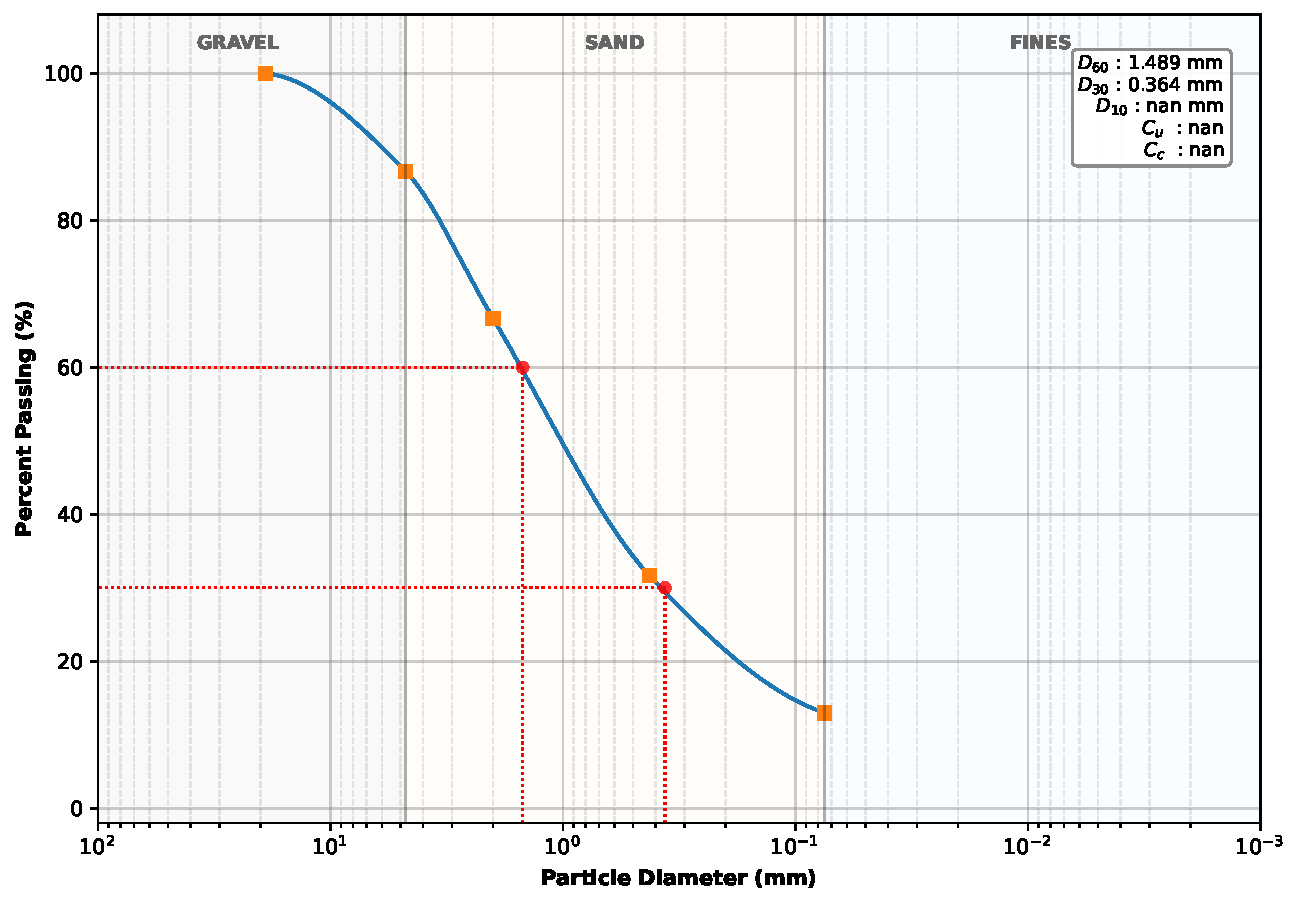
\includegraphics[width=0.85\textwidth]{figures/grain_size.pdf}
\caption{Grain-size distribution generated by
\texttt{ge.grain\_size\_plot()}. Red dashed lines mark $D_{10}$,
$D_{30}$, $D_{60}$ extracted via log-linear interpolation.}
\label{fig:grain}
\end{figure}

\subsection{Diameters and shape coefficients}

\begin{funcbox}{ge.grain\_d10(res) \quad ge.grain\_d30(res) \quad ge.grain\_d60(res)}
Log-linear interpolated $D_x$ values in mm.
\end{funcbox}

\begin{lstlisting}
ge.grain_d10(res), ge.grain_d30(res), ge.grain_d60(res)
\end{lstlisting}
\begin{lstlisting}[style=output]
(0.063, 0.310, 1.520)
\end{lstlisting}

\begin{funcbox}{ge.grain\_Cu(res) \quad ge.grain\_Cc(res)}
\[
C_u = \frac{D_{60}}{D_{10}}, \qquad
C_c = \frac{D_{30}^2}{D_{10}\,D_{60}}.
\]
$C_u \geq 4$ (gravels), $\geq 6$ (sands) and $1 \leq C_c \leq 3$
indicate a well-graded soil.
\end{funcbox}

\begin{lstlisting}
Cu, Cc = ge.grain_Cu(res), ge.grain_Cc(res)
print(f"Cu = {Cu:.2f}, Cc = {Cc:.2f}")
\end{lstlisting}
\begin{lstlisting}[style=output]
Cu = 24.13, Cc = 1.00
\end{lstlisting}

% -----------------------------------------------------------------------
\section{Shear strength}

\subsection{\texttt{ge.direct\_shear(normal, shear, plot=False)}}
\index{direct shear}

\begin{funcbox}{ge.direct\_shear(normal, shear, plot=False)}
Linear regression of peak shear vs.\ normal stress to extract the
Mohr--Coulomb parameters:
\[
\tau_f = c' + \sigmaeff\,\tan\phi'.
\]
\end{funcbox}

\begin{lstlisting}
res = ge.direct_shear(
    normal=[50, 100, 200, 300],
    shear=[35, 65, 125, 185],
)
print(res)
\end{lstlisting}
\begin{lstlisting}[style=output]
{'c': 5.0, 'phi': 31.0, 'R2': 0.999}
\end{lstlisting}

\begin{refbox}
ASTM D3080; Das (2010), Ch.~8.
\end{refbox}

\subsection{\texttt{ge.triaxial(sigma3, delta\_sigma, kind="CD", plot=False)}}
\index{triaxial test}

\begin{funcbox}{ge.triaxial(sigma3, delta\_sigma, kind="CD")}
Process UU / CU / CD triaxial. Computes principal stresses, $p$--$q$
plot points, and the failure-envelope $c', \phi'$.
\end{funcbox}

\begin{lstlisting}
res = ge.triaxial(sigma3=[100, 200, 300], delta_sigma=[180, 280, 380])
print(res)
\end{lstlisting}
\begin{lstlisting}[style=output]
{'c': 10.0, 'phi': 28.5, 'sigma1': [280, 480, 680]}
\end{lstlisting}

\subsection{\texttt{ge.unconfined(qu)}}
\index{unconfined compression}

\begin{funcbox}{ge.unconfined(qu)}
Undrained shear strength from unconfined compression:
\[
S_u = q_u / 2.
\]
\end{funcbox}

\begin{lstlisting}
ge.unconfined(qu=180)
\end{lstlisting}
\begin{lstlisting}[style=output]
{'Su': 90.0}
\end{lstlisting}

\subsection{\texttt{ge.mohr\_circle(sigma1, sigma3, plot=True)}}
\index{Mohr circle}

Plot the Mohr circle of a stress state $(\sigma_1, \sigma_3)$ and
the failure envelope tangent.

% -----------------------------------------------------------------------
\section{Consolidation}

\subsection{\texttt{ge.oedometer(stress, strain)}}
\index{oedometer}

\begin{funcbox}{ge.oedometer(stress, strain)}
Process an $e$--$\log p'$ curve. Returns $C_c$ (compression index)
and $C_r$ (recompression index) by linear regression in their
respective ranges.
\end{funcbox}

\begin{lstlisting}
res = ge.oedometer(
    stress=[25, 50, 100, 200, 400, 800],
    strain=[0.01, 0.03, 0.07, 0.13, 0.19, 0.26]
)
print(f"Cc = {res['Cc']:.3f}, Cr = {res['Cr']:.3f}")
\end{lstlisting}

\begin{refbox}
ASTM D2435.
\end{refbox}

\subsection{\texttt{ge.preconsolidation(e, p, method="casagrande")}}
\index{preconsolidation pressure}

\begin{funcbox}{ge.preconsolidation(e, p, method="casagrande")}
Casagrande's graphical method: bisect the angle between the
tangent at maximum curvature and the horizontal; the
intersection with the backward extension of the virgin
compression line is $\sigma'_p$.
\end{funcbox}

\subsection{\texttt{ge.compression\_index(method, **params)}}
\index{compression index}

\begin{funcbox}{ge.compression\_index(method, **params)}
Empirical correlations for $C_c$. Six methods provided:
\begin{align*}
\textbf{Terzaghi--Peck:} &\quad C_c = 0.009\,(LL - 10) \\
\textbf{Azzouz:}         &\quad C_c = 0.40\,(e_0 - 0.25) \\
\textbf{Skempton:}       &\quad C_c = 0.007\,(LL - 7) \\
\textbf{Hough:}          &\quad C_c = 0.30\,(e_0 - 0.27) \\
\textbf{Rendon-Herrero:} &\quad C_c = 0.141\,G_s^{1.2}\bigl((1+e_0)/G_s\bigr)^{2.38} \\
\textbf{Nagaraj-Murty:}  &\quad C_c = 0.2343\,(LL/100)\,G_s
\end{align*}
\end{funcbox}

\begin{lstlisting}
ge.compression_index(method="terzaghi_peck", LL=48)
ge.compression_index(method="azzouz", e0=0.92)
\end{lstlisting}
\begin{lstlisting}[style=output]
0.342
0.268
\end{lstlisting}

\subsection{\texttt{ge.cv(t, deformation, method="root\_time")}}
\index{coefficient of consolidation}

\begin{funcbox}{ge.cv(t, deformation, method="root\_time")}
\textbf{Root-time (Taylor 1948):}
$c_v = T_{90}\,H_{dr}^2/t_{90}$ with $T_{90} = 0.848$.\\
\textbf{Log-time (Casagrande):}
$c_v = T_{50}\,H_{dr}^2/t_{50}$ with $T_{50} = 0.197$.
\end{funcbox}

% -----------------------------------------------------------------------
\section{Compaction}

\subsection{\texttt{ge.proctor(water\_content, dry\_density)}}
\index{Proctor compaction}

\begin{funcbox}{ge.proctor(water\_content, dry\_density)}
Fit a parabola to the $(w, \gamma_d)$ points and locate the peak.
Returns $w_{\text{opt}}$ (\%) and $\gamma_{d,\max}$ (kN/m\textsuperscript{3}).
\end{funcbox}

\begin{lstlisting}
res = ge.proctor(
    water_content=[10, 12, 14, 16, 18, 20],
    dry_density=[16.5, 17.2, 17.85, 17.65, 17.1, 16.4],
)
print(res)
\end{lstlisting}
\begin{lstlisting}[style=output]
{'w_opt': 14.4, 'gamma_d_max': 17.87, 'fit_R2': 0.998}
\end{lstlisting}

\begin{refbox}
ASTM D698 (Standard); ASTM D1557 (Modified).
\end{refbox}

\subsection{\texttt{ge.proctor\_plot(...)}}

\begin{lstlisting}
ge.proctor_plot(
    water_content=[10, 12, 14, 16, 18, 20],
    dry_density=[16.5, 17.2, 17.85, 17.65, 17.1, 16.4],
    Gs=2.70, show_zav=True,
    save_as="proctor.pdf",
)
\end{lstlisting}

\begin{figure}[h]\centering
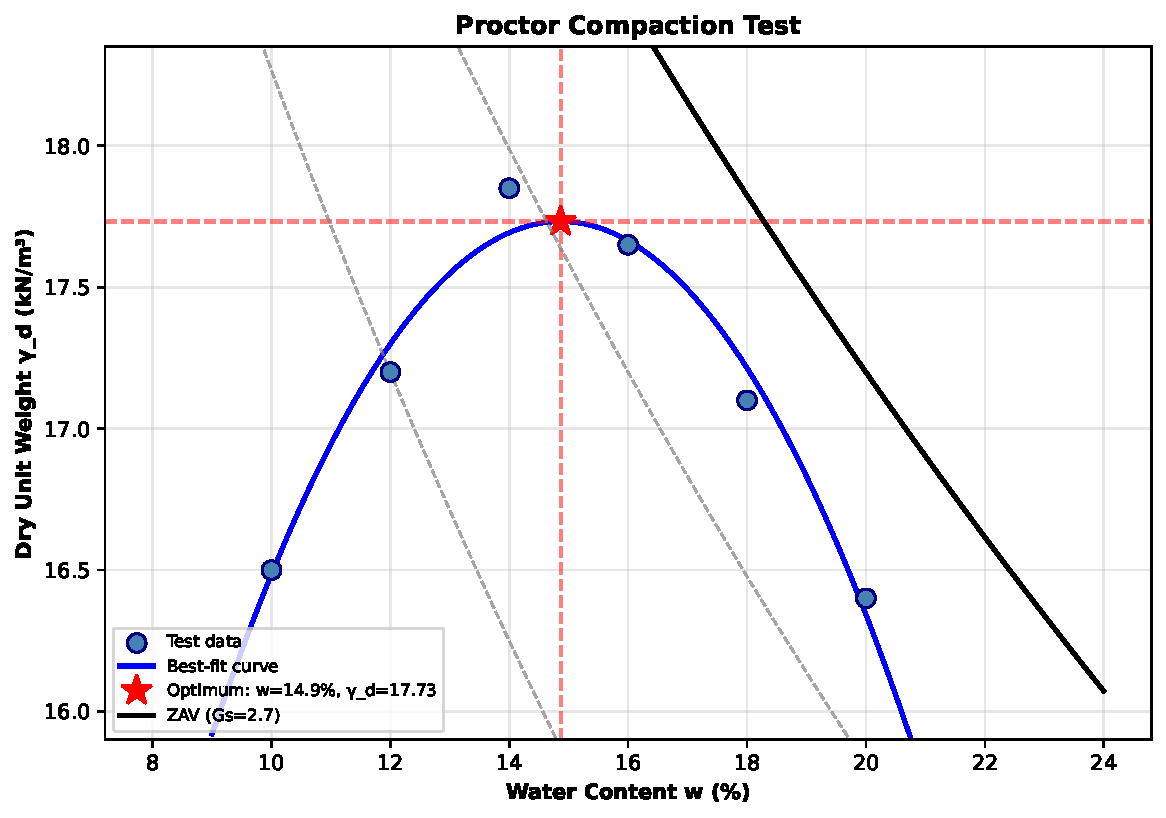
\includegraphics[width=0.78\textwidth]{figures/proctor.pdf}
\caption{Proctor compaction curve generated by
\texttt{ge.proctor\_plot()}. The zero-air-voids line
($\gamma_d^{\text{zav}} = G_s\gammaw / (1 + wG_s)$) is shown for
$G_s = 2.70$.}
\label{fig:proctor}
\end{figure}

\subsection{\texttt{ge.zav\_line(Gs, w\_range)}}

\begin{funcbox}{ge.zav\_line(Gs, w\_range)}
Zero-air-voids line:
\[
\gamma_d^{\text{zav}}(w) = \frac{G_s\,\gammaw}{1 + w\,G_s}.
\]
\end{funcbox}

\subsection{\texttt{ge.relative\_compaction(gamma\_d, gamma\_d\_max)}}

\begin{lstlisting}
ge.relative_compaction(gamma_d=17.2, gamma_d_max=17.87)
\end{lstlisting}
\begin{lstlisting}[style=output]
96.25   # percent
\end{lstlisting}

% -----------------------------------------------------------------------
\section{Permeability and CBR}

\subsection{\texttt{ge.constant\_head(L, A, Q, t, h)}}
\index{permeability!constant head}

\begin{funcbox}{ge.constant\_head(L, A, Q, t, h)}
\[
k = \frac{Q\,L}{A\,h\,t}\quad[\si{\meter\per\second}].
\]
\end{funcbox}

\begin{lstlisting}
ge.constant_head(L=0.15, A=8.2e-3, Q=4.5e-4, t=60, h=0.30)
\end{lstlisting}
\begin{lstlisting}[style=output]
4.57e-05   # m/s -> sandy soil
\end{lstlisting}

\subsection{\texttt{ge.falling\_head(L, a, A, t, h1, h2)}}

\begin{funcbox}{ge.falling\_head(L, a, A, t, h1, h2)}
\[
k = \frac{a\,L}{A\,t}\ln\!\left(\frac{h_1}{h_2}\right).
\]
\end{funcbox}

\subsection{\texttt{ge.cbr\_test(penetration, load)}}
\index{CBR}

\begin{funcbox}{ge.cbr\_test(penetration, load)}
California Bearing Ratio at 2.54~mm and 5.08~mm penetration,
normalised against standard crushed-stone reactions
(13.24~kN at 2.54~mm; 19.96~kN at 5.08~mm).
\end{funcbox}

\begin{lstlisting}
res = ge.cbr_test(penetration=[0, 0.5, 1.0, 2.54, 5.08, 7.62],
                   load=[0, 1.2, 2.8, 4.4, 7.2, 9.0])
print(res)
\end{lstlisting}
\begin{lstlisting}[style=output]
{'CBR_2.54': 33.2, 'CBR_5.08': 36.1, 'CBR_design': 36.1}
\end{lstlisting}

% ============================================================================
%  CHAPTER 4 -- SITE INVESTIGATION
% ============================================================================
\chapter{Site Investigation}\label{ch:site}

\epigraph{Lab tests answer the question:
``what does the soil do under these stresses?''
Site investigation answers:
``what stresses can we actually deliver to this soil?''}{}

\noindent
This chapter is the largest in the book and covers eight families
of in-situ tests. For each, GeoEq provides the unit-conversion
and correlation library that turns raw field readings into the
parameters consumed downstream by Chapters
\ref{ch:stress}--\ref{ch:dynamics}.

% -----------------------------------------------------------------------
\section{Standard Penetration Test (SPT)}\label{sec:spt}

\subsection{\texttt{ge.spt\_n60(N, ER, Cb=1, Cs=1, Cr=1)}}\index{SPT!energy correction}

\begin{funcbox}{ge.spt\_n60(N, ER, Cb=1, Cs=1, Cr=1)}
Energy-corrected blow count:
\[
N_{60} = N \cdot \frac{ER}{60} \cdot C_b \cdot C_s \cdot C_r,
\]
where $ER$ is field energy ratio, $C_b$ borehole-diameter, $C_s$
sampler, $C_r$ rod-length corrections.
\end{funcbox}

\begin{lstlisting}
ge.spt_n60(N=18, ER=72, Cb=1.0, Cs=1.0, Cr=0.95)
\end{lstlisting}
\begin{lstlisting}[style=output]
20.52
\end{lstlisting}

\begin{refbox}
Skempton (1986); Seed et al.\ (1985).
\end{refbox}

\subsection{\texttt{ge.spt\_n160(N60, sigma\_v, method="liao\_whitman")}}

\begin{funcbox}{ge.spt\_n160(N60, sigma\_v, method)}
Overburden-corrected blow count $(N_1)_{60} = C_N\,N_{60}$:
\begin{align*}
\textbf{Liao--Whitman (1986):}      & \quad C_N = \sqrt{p_a / \sigmavp},\;\; C_N \leq 2 \\
\textbf{Skempton (1986), sand:}     & \quad C_N = \tfrac{2}{1 + \sigmavp/p_a} \\
\textbf{Peck--Hanson--Thornburn:}   & \quad C_N = 0.77\,\log_{10}(2000/\sigmavp')
\end{align*}
\end{funcbox}

\begin{lstlisting}
ge.spt_n160(N60=18, sigma_v=120, method="liao_whitman")
\end{lstlisting}
\begin{lstlisting}[style=output]
16.55
\end{lstlisting}

\subsection{\texttt{ge.spt\_n160cs(N160, FC)}}

\begin{funcbox}{ge.spt\_n160cs(N160, FC)}
Fines-content correction for liquefaction:
$(N_1)_{60,cs} = \alpha + \beta(N_1)_{60}$
with $\alpha, \beta$ piecewise-linear in fines content $FC$.
\end{funcbox}

\subsection{\texttt{ge.spt\_friction\_angle(N, sigma\_v, method)}}

\begin{funcbox}{ge.spt\_friction\_angle(N, sigma\_v, method)}
Three correlations:
\begin{align*}
\textbf{Hatanaka--Uchida (1996):} & \quad \phi' = \sqrt{20\,(N_1)_{60}} + 20 \\
\textbf{Kulhawy--Mayne (1990):}   & \quad \phi' = \tan^{-1}\!\left[
                                    \tfrac{N_{60}}{12.2 + 20.3(\sigmavp/p_a)}\right]^{0.34} \\
\textbf{Peck--Hanson--Thornburn:} & \quad \phi' = 27.1 + 0.30 N - 5.4\cdot10^{-4} N^2
\end{align*}
\end{funcbox}

\begin{lstlisting}
ge.spt_friction_angle(N=15, sigma_v=80, method="hatanaka")
\end{lstlisting}
\begin{lstlisting}[style=output]
33.2   # degrees
\end{lstlisting}

\subsection{\texttt{ge.spt\_su(N60, method, PI)}}

\begin{funcbox}{ge.spt\_su(N60, method, PI)}
\begin{align*}
\textbf{Stroud (1974):} & \quad S_u = f_1\,N_{60},\quad f_1 \in [4,6] \\
\textbf{Hara (1974):}   & \quad S_u = 29\,N_{60}^{0.72}
\end{align*}
\end{funcbox}

\subsection{\texttt{ge.spt\_dr(N160, method="meyerhof")} and \texttt{ge.spt\_modulus(...)}}

Relative density and elastic modulus correlations: Meyerhof,
Skempton, Kulhawy--Mayne (1990) for $D_r$; Bowles (1996) for $E_s$
across six soil categories.

% -----------------------------------------------------------------------
\section{Cone Penetration Test (CPT)}\label{sec:cpt}

\subsection{Normalisation --- \texttt{ge.cpt\_normalize(...)}}

\begin{funcbox}{ge.cpt\_normalize(qt, fs, sigma\_v, sigma\_v\_eff, u2, u0=0)}
Robertson 2009 normalised parameters:
\begin{align}
Q_t &= \frac{q_t - \sigmav}{\sigmavp} \\
F_r &= \frac{f_s}{q_t - \sigmav}\cdot 100\% \\
B_q &= \frac{u_2 - u_0}{q_t - \sigmav}
\end{align}
\end{funcbox}

\begin{lstlisting}
Qt, Fr, Bq = ge.cpt_normalize(qt=4.2, fs=0.05, sigma_v=80,
                                sigma_v_eff=50, u2=120, u0=50)
print(Qt, Fr, Bq)
\end{lstlisting}
\begin{lstlisting}[style=output]
82.40  1.21  16.99
\end{lstlisting}

\subsection{\texttt{ge.cpt\_ic(Qt, Fr)} and \texttt{ge.cpt\_sbt(Qt, Fr)}}
\index{CPT!Ic}\index{CPT!SBT}

\begin{funcbox}{ge.cpt\_ic(Qt, Fr)}
Soil-behaviour-type index:
\[
I_c = \sqrt{(3.47 - \log_{10} Q_t)^2 + (\log_{10} F_r + 1.22)^2}.
\]
\end{funcbox}

\begin{lstlisting}
ge.cpt_ic(Qt=80, Fr=1.2)
\end{lstlisting}
\begin{lstlisting}[style=output]
1.951   # SBT zone 6, 'Sands - clean sand to silty sand'
\end{lstlisting}

\subsection{\texttt{ge.cpt\_sbt\_plot(Qt, Fr)}}

\begin{lstlisting}
ge.cpt_sbt_plot(Qt=[8, 25, 80, 150], Fr=[5.0, 2.5, 1.2, 0.5],
                save_as="cpt_sbt.pdf")
\end{lstlisting}

\begin{figure}[h]\centering
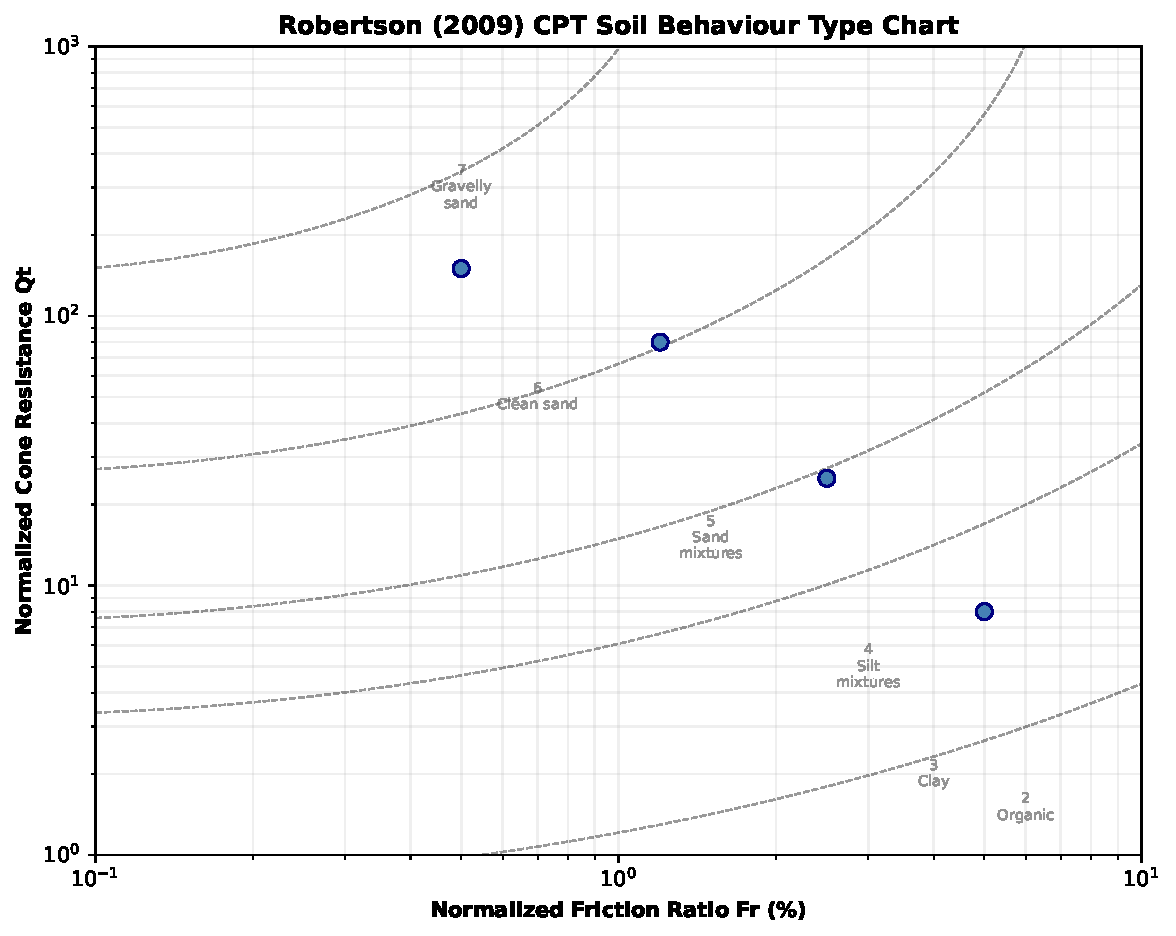
\includegraphics[width=0.8\textwidth]{figures/cpt_sbt.pdf}
\caption{Robertson (1990) soil-behaviour-type chart with four
CPT data points overlaid. Generated by \texttt{ge.cpt\_sbt\_plot()}.}
\label{fig:cpt_sbt}
\end{figure}

\subsection{Correlations: $\phi'$, $S_u$, $D_r$, $M$}

\begin{lstlisting}
ge.cpt_friction_angle(qt=4.2, sigma_v_eff=50)       # Robertson-Campanella
ge.cpt_su(qt=4.2, sigma_v=80, Nkt=15)               # Lunne et al.
ge.cpt_dr(qc=4.2, sigma_v_eff=50)                   # Baldi et al.
ge.cpt_modulus(qt=4.2, sigma_v=80, Ic=1.95)         # Robertson 2009
\end{lstlisting}

% -----------------------------------------------------------------------
\section{Field vane shear, pressuremeter, plate-load, pile-load tests}

This section consolidates the four families.

\subsection{Field vane --- \texttt{ge.vane\_su(T, D, H)}}

\begin{funcbox}{ge.vane\_su(T, D, H)}
Undrained shear strength from a rectangular vane:
\[
S_u = \frac{T}{\pi D^2\,(H/2 + D/6)}.
\]
\end{funcbox}

\begin{lstlisting}
ge.vane_su(T=85, D=0.065, H=0.130)   # T in N.m, D, H in m
\end{lstlisting}
\begin{lstlisting}[style=output]
52.3   # kPa
\end{lstlisting}

\subsection{Bjerrum correction --- \texttt{ge.vane\_correction(Su, PI)}}

\begin{funcbox}{ge.vane\_correction(Su\_fvt, PI)}
Bjerrum (1972): $\mu_R$ vs.\ PI, reducing FVT $S_u$ to design.
\end{funcbox}

\subsection{Pressuremeter --- \texttt{ge.pmt\_parameters / pmt\_su / pmt\_modulus ...}}

The six pressuremeter functions cover modulus, limit pressure,
$S_u$, bearing capacity, settlement, and $K_0$ extraction per
M\'enard (1975) and Baguelin et al.\ (1978).

\subsection{Plate-load test --- \texttt{ge.plt\_bearing / ge.plt\_subgrade\_modulus / ...}}

Three failure criteria (log-log break, tangent intersection,
settlement); Terzaghi--Peck size correction for scaling plate
results to a real footing.

\subsection{Pile-load-test interpretation (nine methods)}
\index{Davisson}\index{Chin}

\begin{funcbox}{ge.davisson(load, settlement, D, L, A, E)}
Davisson's offset limit: ultimate at the intersection of the
load--settlement curve with the line
$s = PL/AE + (4 + D/120)~\text{mm}$.
\end{funcbox}

\begin{funcbox}{ge.chin(load, settlement)}
Chin's hyperbolic method: plot $s/Q$ vs.\ $s$; ultimate $= 1/$slope.
\end{funcbox}

Plus De Beer, Hansen 80\%, FHWA 5\%, Case method, Hiley,
Danish formula, and ENR.

\begin{lstlisting}
loads = [0, 100, 250, 500, 800, 1100, 1400]
sett  = [0,   1,   3,    7,   14,   25,   45]
Qu_dav  = ge.davisson(loads, sett, D=0.4, L=15, A=0.126, E=30e6)
Qu_chin = ge.chin(loads, sett)
print(Qu_dav, Qu_chin)
\end{lstlisting}

% -----------------------------------------------------------------------
\section{Field permeability and DCP}

\begin{funcbox}{ge.slug\_test(r, R, Le, T0)}
Hvorslev (1951) slug-test permeability:
\[
k = \frac{r^2 \ln(2 L_e / R)}{2 L_e\,T_0}.
\]
\end{funcbox}

\begin{funcbox}{ge.pumping\_test\_confined(Q, h1, h2, r1, r2, H)}
Thiem (confined): $k = \dfrac{Q\,\ln(r_2/r_1)}{2\pi H (h_2 - h_1)}$.
\end{funcbox}

\begin{funcbox}{ge.dcp\_cbr(dcpi, method="webster")}\index{DCP}
Three correlations:
\begin{align*}
\textbf{Webster (1992):} &\quad \log_{10}\text{CBR} = 2.465 - 1.12\log_{10}\text{DCPI} \\
\textbf{TRL (1990):}     &\quad \log_{10}\text{CBR} = 2.48 - 1.057\log_{10}\text{DCPI} \\
\textbf{Kleyn (1975):}   &\quad \log_{10}\text{CBR} = 2.628 - 1.273\log_{10}\text{DCPI}
\end{align*}
\end{funcbox}

% ============================================================================
%  CHAPTER 5 -- LAYERED PROFILES
% ============================================================================
\chapter{Layered Soil Profiles}\label{ch:profile}

\epigraph{In a one-line profile the stress is trivial.
In a real one, it never is.}{}

\subsection*{\texttt{ge.Soil} and \texttt{ge.SoilProfile}}

The \texttt{Soil} dataclass holds one homogeneous layer; a
\texttt{SoilProfile} stacks layers and integrates unit weights
downward to compute total, pore, and effective stress at any
depth.

\begin{funcbox}{ge.Soil(name, gamma=18.0, gamma\_sat=None, phi=30, c=0, e=None, Gs=2.70, k=None, Es=None, mu=0.30, Cc=None, Cr=None, OCR=1.0, Su=None)}
A plain dataclass. Only \texttt{name} is required. \texttt{gamma\_sat}
defaults to $\gamma + 1.5$ if not given. Method
\texttt{.gamma\_effective()} returns $\gamma' = \gamma_{\text{sat}}
- \gammaw$.
\end{funcbox}

\begin{funcbox}{ge.SoilProfile(layers, water\_table=None)}
\textbf{Stress at depth} ($\text{Das 2010 Ch.\ 5}$):
\begin{align}
\sigmav(z)  &= \sum_i \gamma_i\,\Delta z_i \\
u(z)        &= \gammaw \max(0,\; z - z_w) \\
\sigmavp(z) &= \sigmav(z) - u(z)
\end{align}
\textbf{Methods:} \texttt{total\_stress(z)},
\texttt{pore\_pressure(z)}, \texttt{effective\_stress(z)},
\texttt{stress\_at(z)}, \texttt{layer\_at(z)},
\texttt{add\_layer(top, bot, soil)}, \texttt{to\_dataframe()},
\texttt{plot(dz=0.1)}.
\end{funcbox}

\begin{worked}{Three-layer profile with intermediate water table}
\begin{lstlisting}
clay = ge.Soil("Soft Clay", gamma=17, gamma_sat=18.5,
               phi=0, c=25, e=0.9)
sand = ge.Soil("Dense Sand", gamma=19, gamma_sat=20.5, phi=35)

p = ge.SoilProfile([
    (0, 2,  ge.Soil("Fill", gamma=18)),
    (2, 8,  clay),
    (8, 20, sand),
], water_table=1.5)

print(p.stress_at(10))     # at the middle of the sand
print(p.layer_at(5).name)
p.plot(dz=0.1, save_as="profile_stress.pdf")
\end{lstlisting}
\begin{lstlisting}[style=output]
{'sigma': 188.0, 'u': 78.48, 'sigma_eff': 109.52}
Soft Clay
\end{lstlisting}
\end{worked}

\begin{figure}[h]\centering
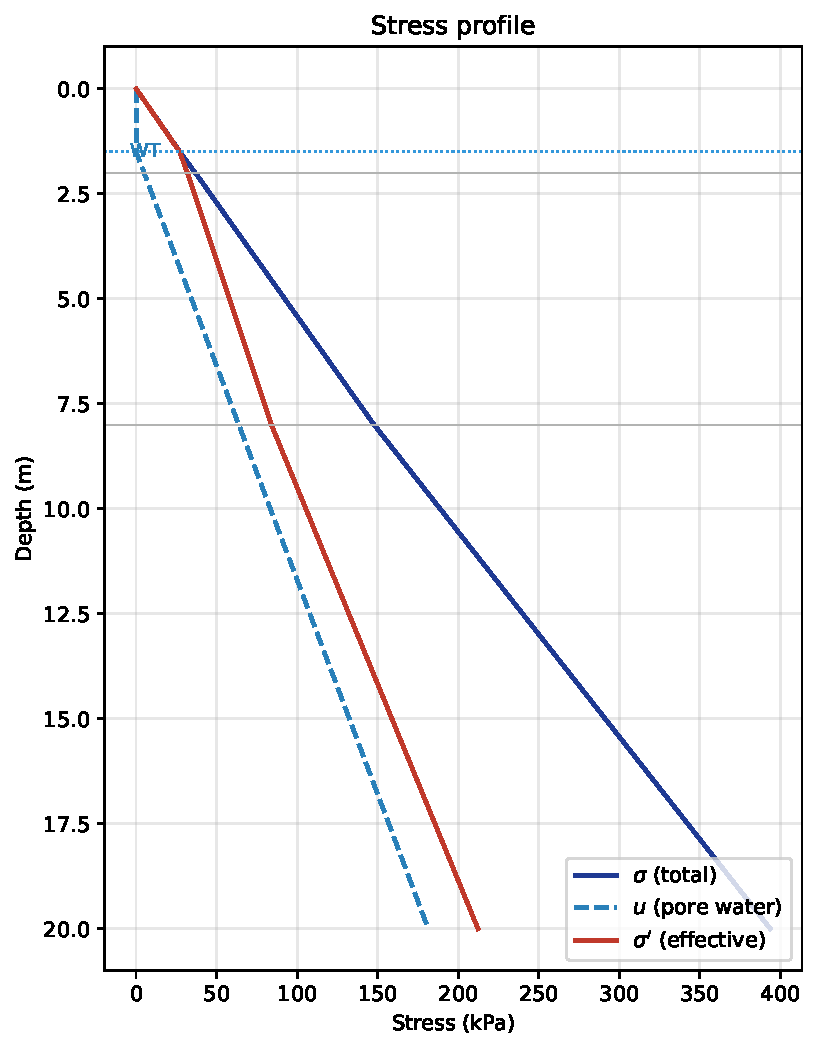
\includegraphics[width=0.65\textwidth]{figures/profile_stress.pdf}
\caption{Total, pore, and effective vertical stress vs depth for
a three-layer profile (Fill / Soft Clay / Dense Sand) with the
water table at 1.5~m. Generated by \texttt{SoilProfile.plot()}.}
\label{fig:profile}
\end{figure}

\begin{funcbox}{ge.mesh(profile, dz=0.5) \quad ge.log\_plot(boreholes)}
\texttt{mesh} returns a depth grid spanning the profile;
\texttt{log\_plot} renders a multi-borehole log given
\texttt{\{label: profile\}}.
\end{funcbox}

% ============================================================================
%  CHAPTER 6 -- EFFECTIVE STRESS AND SEEPAGE
% ============================================================================
\chapter{Effective Stress and Seepage}\label{ch:stress}

\epigraph{The principle of effective stress is the single most
useful equation in soil mechanics, and the one most casually
mis-applied.}{}

% -----------------------------------------------------------------------
\section{Effective stress}

\subsection{\texttt{ge.total\_stress(gamma, depth)}}

\begin{funcbox}{ge.total\_stress(gamma, depth)}
\[
\sigmav = \sum_i \gamma_i\,H_i.
\]
\texttt{gamma}, \texttt{depth} are scalars (single layer) or
matching sequences (multiple layers).
\end{funcbox}

\begin{lstlisting}
ge.total_stress(18.0, 5.0)
ge.total_stress([17, 19, 20], [2, 3, 5])
\end{lstlisting}
\begin{lstlisting}[style=output]
90.0
191.0
\end{lstlisting}

\subsection{\texttt{ge.pore\_pressure(z, z\_w=0, gamma\_w=9.81)}}

\begin{funcbox}{ge.pore\_pressure(z, z\_w=0)}
\[
u = \gammaw\,\max(0, z - z_w).
\]
Accepts scalar or NumPy-array \texttt{z}.
\end{funcbox}

\begin{lstlisting}
ge.pore_pressure(5.0, z_w=2.0)
ge.pore_pressure([0, 2, 5, 10], z_w=2)
\end{lstlisting}
\begin{lstlisting}[style=output]
29.43
array([ 0.  ,  0.  , 29.43, 78.48])
\end{lstlisting}

\subsection{\texttt{ge.effective\_stress(sigma, u)}}

\begin{funcbox}{ge.effective\_stress(sigma, u)}
Terzaghi's principle: $\sigmaeff = \sigmav - u$. Scalar or array.
\end{funcbox}

\begin{lstlisting}
ge.effective_stress(154.0, 58.86)
\end{lstlisting}
\begin{lstlisting}[style=output]
95.14
\end{lstlisting}

\subsection{\texttt{ge.capillary\_rise(D10, e, C=0.2)}}

\begin{funcbox}{ge.capillary\_rise(D10, e, C=0.2)}
Hazen-type estimate, returns metres:
$h_c = C / (e\, D_{10}^{\text{cm}})$.
\end{funcbox}

\begin{lstlisting}
ge.capillary_rise(D10=0.05, e=0.7)
\end{lstlisting}
\begin{lstlisting}[style=output]
0.5714   # ~57 cm of capillary rise in a fine sand
\end{lstlisting}

% -----------------------------------------------------------------------
\section{Seepage}

\begin{funcbox}{ge.darcy\_flow(k, i, A)}
$Q = k\,i\,A$.
\end{funcbox}

\begin{lstlisting}
ge.darcy_flow(k=1e-4, i=0.1, A=1.0)
\end{lstlisting}
\begin{lstlisting}[style=output]
1.0e-05    # m^3/s
\end{lstlisting}

\begin{funcbox}{ge.hydraulic\_gradient(dh, L)}
$i = \Delta h / L$.
\end{funcbox}

\begin{funcbox}{ge.critical\_gradient(Gs, e)}
$i_{\text{cr}} = (G_s - 1)/(1 + e)$. Quicksand / heave when upward
$i \geq i_{\text{cr}}$.
\end{funcbox}

\begin{lstlisting}
ge.critical_gradient(Gs=2.65, e=0.65)
\end{lstlisting}
\begin{lstlisting}[style=output]
1.0   # the classic textbook answer
\end{lstlisting}

\begin{funcbox}{ge.equivalent\_k(k\_layers, H\_layers, direction)}
\textbf{Horizontal (parallel flow):}
$k_{\text{eq}}^{H} = \dfrac{\sum k_i H_i}{\sum H_i}$.\\
\textbf{Vertical (series flow):}
$k_{\text{eq}}^{V} = \dfrac{\sum H_i}{\sum H_i / k_i}$.
\end{funcbox}

\begin{lstlisting}
ge.equivalent_k([1e-3, 1e-5], [5, 5], direction="horizontal")
ge.equivalent_k([1e-3, 1e-5], [5, 5], direction="vertical")
\end{lstlisting}
\begin{lstlisting}[style=output]
5.05e-04    # arithmetic average dominates
1.98e-05    # harmonic-like; lowest k dominates
\end{lstlisting}

\begin{warnbox}
Layered seepage is anisotropic by orders of magnitude. The
horizontal $k$ above is \emph{25 times} the vertical $k$ for the
same two layers --- this is the engineering case for filter
drains and not for impermeable cores.
\end{warnbox}

\begin{funcbox}{ge.flow\_net(Nf, Nd, k, dh, L=1)}
$Q = k\,\Delta h\,(N_f/N_d)\,L$ per metre normal to the flow plane.
\end{funcbox}

\begin{lstlisting}
ge.flow_net(Nf=4, Nd=8, k=1e-5, dh=10)
\end{lstlisting}
\begin{lstlisting}[style=output]
5.0e-05    # m^3/s per metre of cut-off wall
\end{lstlisting}

% ============================================================================
%  CHAPTER 7 -- STRESS DISTRIBUTION
% ============================================================================
\chapter{Stress Distribution Beneath Loads}\label{ch:boussinesq}

\section{Boussinesq family}

\subsection{\texttt{ge.boussinesq\_point(P, z, r=0)}}\index{Boussinesq!point load}

\begin{funcbox}{ge.boussinesq\_point(P, z, r=0)}
Stress beneath a concentrated load on a semi-infinite elastic mass:
\[
\Delta\sigma_z = \frac{3P}{2\pi z^2}\cdot
\frac{1}{[1 + (r/z)^2]^{5/2}}.
\]
\end{funcbox}

\begin{lstlisting}
ge.boussinesq_point(P=100, z=2, r=0)
ge.boussinesq_point(P=100, z=2, r=3)
\end{lstlisting}
\begin{lstlisting}[style=output]
11.94    # directly below the load
0.66     # 3 m laterally
\end{lstlisting}

\begin{lstlisting}
ge.stress_isobar_plot(P=100, save_as="stress_bulb.pdf")
\end{lstlisting}

\begin{figure}[h]\centering
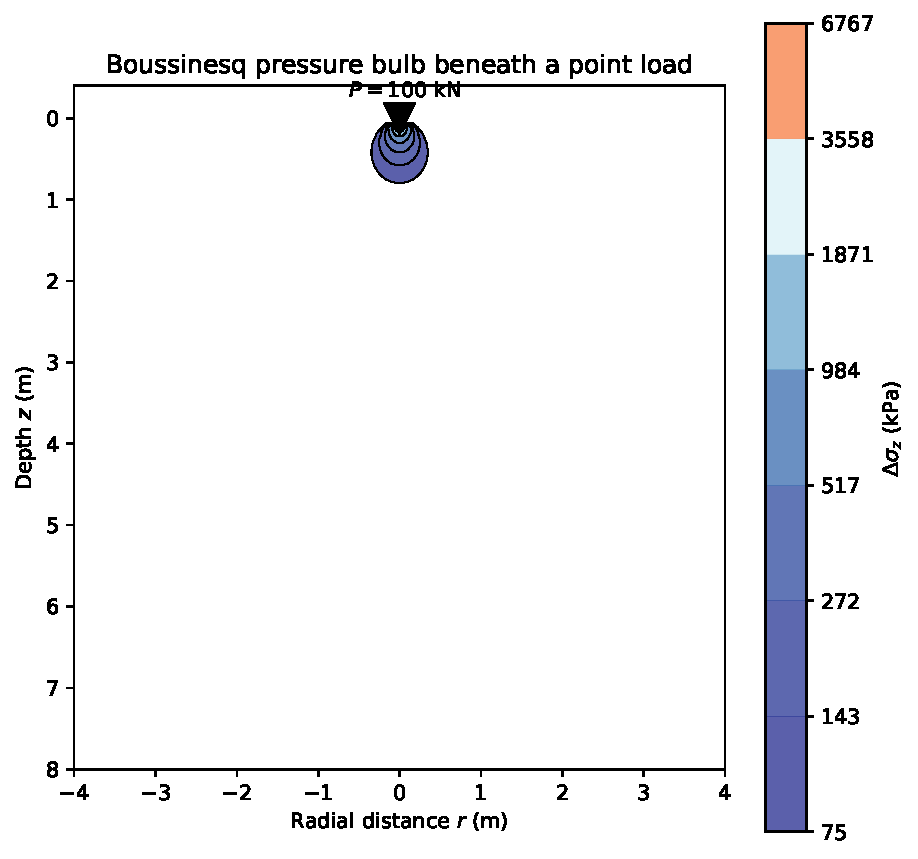
\includegraphics[width=0.55\textwidth]{figures/stress_bulb.pdf}
\caption{Pressure bulb under a 100~kN point load, computed from
the Boussinesq solution and plotted by
\texttt{ge.stress\_isobar\_plot()}.}
\label{fig:bulb}
\end{figure}

\subsection{Line, strip, circular, rectangular loads}

\begin{funcbox}{ge.boussinesq\_line(q, z, x=0)}
$\Delta\sigma_z = \tfrac{2q}{\pi z}\cdot \tfrac{1}{[1 + (x/z)^2]^2}.$
\end{funcbox}

\begin{funcbox}{ge.boussinesq\_strip(q, B, z, x=0)}
$\Delta\sigma_z = \tfrac{q}{\pi}\bigl[\alpha + \sin\alpha\cos(\alpha + 2\beta)\bigr]$
with $\alpha, \beta$ the angles subtended at the point by the
strip edges.
\end{funcbox}

\begin{funcbox}{ge.boussinesq\_circular(q, R, z)}
Centreline stress under a uniformly loaded circle:
\[
\Delta\sigma_z = q\!\left[1 - \frac{1}{(1 + (R/z)^2)^{3/2}}\right].
\]
\end{funcbox}

\begin{lstlisting}
ge.boussinesq_circular(q=100, R=2, z=2)
\end{lstlisting}
\begin{lstlisting}[style=output]
64.65    # Das Table 6.6: dsigma/q = 0.6465 at z = R
\end{lstlisting}

\subsection{Newmark / Fadum influence value}

\begin{funcbox}{ge.newmark\_influence(m, n)}\index{Newmark!influence}
With $m = B/z$, $n = L/z$:
\[
I = \frac{1}{4\pi}\!\left\{
\frac{2mn\sqrt{m^2+n^2+1}}{m^2+n^2+m^2n^2+1}\cdot
\frac{m^2+n^2+2}{m^2+n^2+1}
+ \tan^{-1}\!\left[\frac{2mn\sqrt{m^2+n^2+1}}{m^2+n^2-m^2n^2+1}\right]\right\}.
\]
\end{funcbox}

\begin{lstlisting}
ge.newmark_influence(m=1.0, n=1.0)    # Das Table 6.5
\end{lstlisting}
\begin{lstlisting}[style=output]
0.1752
\end{lstlisting}

\begin{funcbox}{ge.boussinesq\_rect(q, B, L, z, position="corner")}
Uses Fadum's $I$ with superposition for centre / edge / corner.
\end{funcbox}

\subsection{\texttt{ge.westergaard\_point(P, z, r=0, mu=0)}}\index{Westergaard}

\begin{funcbox}{ge.westergaard\_point(P, z, r=0, mu=0)}
Westergaard's stratified-medium solution:
\[
\Delta\sigma_z = \frac{P}{\pi z^2}\cdot
\frac{\eta}{[\eta^2 + (r/z)^2]^{3/2}},\quad
\eta = \sqrt{\tfrac{1 - 2\mu}{2 - 2\mu}}.
\]
\end{funcbox}

\subsection{\texttt{ge.stress\_2to1(q, B, L, z)}}

\begin{funcbox}{ge.stress\_2to1(q, B, L, z)}
2:1 spreading approximation:
$\Delta\sigma_z = qBL/[(B+z)(L+z)]$.
Useful for quick estimates above $z \sim 2B$.
\end{funcbox}

\begin{lstlisting}
ge.stress_2to1(q=100, B=2, L=4, z=5)
\end{lstlisting}
\begin{lstlisting}[style=output]
12.70
\end{lstlisting}

% ============================================================================
%  CHAPTER 8 -- BEARING CAPACITY
% ============================================================================
\chapter{Bearing Capacity}\label{ch:bearing}

\epigraph{Terzaghi solved the bearing-capacity equation in 1943.
The profession has been arguing about $N_\gamma$ ever since.}{}

\noindent
The general bearing-capacity equation (Meyerhof / Hansen / Vesic):
\begin{equation}\label{eq:bearing}
\boxed{\;q_u = c\,N_c\,s_c\,d_c\,i_c
         + q\,N_q\,s_q\,d_q\,i_q
         + \tfrac{1}{2}\gamma B\,N_\gamma\,s_\gamma\,d_\gamma\,i_\gamma\;}
\end{equation}
Terzaghi (1943) uses the same first/second/third-term form but
without shape, depth, or inclination corrections.

\section{Bearing factors}

\subsection{\texttt{ge.bearing\_factors(phi, method)}}

\begin{funcbox}{ge.bearing\_factors(phi, method)}
Closed-form $N_c, N_q, N_\gamma$:
\begin{align}
N_q &= e^{\pi\tan\phi}\,\tan^2(45^\circ + \phi/2) \\
N_c &= (N_q - 1)\cot\phi \quad\text{(}5.14\text{ at }\phi = 0\text{)}\\
N_\gamma &= \begin{cases}
(N_q - 1)\tan(1.4\phi) & \text{Meyerhof}\\
1.5(N_q - 1)\tan\phi   & \text{Hansen}\\
2(N_q + 1)\tan\phi     & \text{Vesic}
\end{cases}
\end{align}
\end{funcbox}

\begin{lstlisting}
ge.bearing_factors(phi=30, method="meyerhof")
\end{lstlisting}
\begin{lstlisting}[style=output]
{'Nc': 30.14, 'Nq': 18.40, 'Ngamma': 15.67}
\end{lstlisting}

\begin{table}[h]\centering
\caption{Bearing-capacity factors at selected $\phi$ (computed by
\texttt{ge.bearing\_factors}).}
\label{tab:Nfactors}
\small
\begin{tabular}{rrrrrr}\toprule
$\phi^\circ$ & $N_c$ & $N_q$ & $N_\gamma^{\text{Meyerhof}}$ &
$N_\gamma^{\text{Hansen}}$ & $N_\gamma^{\text{Vesic}}$\\\midrule
0  & 5.14  & 1.00  & 0.00  & 0.00  & 0.00\\
20 & 14.83 & 6.40  & 2.87  & 2.95  & 5.39\\
30 & 30.14 & 18.40 & 15.67 & 14.39 & 22.40\\
40 & 75.31 & 64.20 & 93.69 & 79.54 & 109.41\\
\bottomrule
\end{tabular}
\end{table}

\section{Shape, depth, and inclination factors}

\begin{funcbox}{ge.bearing\_shape\_factors(B, L, phi, method)}
\textbf{Meyerhof:} $s_c = 1 + 0.2 K_p (B/L)$, $s_q = s_\gamma =
1 + 0.1 K_p (B/L)$ for $\phi \geq 10°$.\\
\textbf{Hansen / Vesic:} $s_c = 1 + (N_q/N_c)(B/L)$,
$s_q = 1 + (B/L)\tan\phi$,
$s_\gamma = \max(0.6,\, 1 - 0.4(B/L))$.
\end{funcbox}

\begin{funcbox}{ge.bearing\_depth\_factors(Df, B, phi, method)}
Meyerhof: $d_c = 1 + 0.2\sqrt{K_p}(D_f/B)$, $d_q = d_\gamma = 1
+ 0.1\sqrt{K_p}(D_f/B)$ for $\phi \geq 10°$.\\
Hansen / Vesic: piecewise-linear $k$-factor.
\end{funcbox}

\begin{funcbox}{ge.bearing\_inclination\_factors(beta, phi, c, method)}
$i_c = i_q = (1 - \beta/90)^2$; $i_\gamma = (1 - \beta/\phi)^2$.
\end{funcbox}

\section{Ultimate and allowable capacity}

\begin{funcbox}{ge.bearing\_capacity(c, gamma, Df, B, phi, L=None, method="meyerhof", shape=True, depth=True, inclination=0, water\_table="deep")}
Computes Eq.~\ref{eq:bearing} with all selectable corrections.
Returns a dict with \texttt{q\_u}, the factors used, and the
method name.
\end{funcbox}

\begin{worked}{Square footing on dense sand}
A 2~m square footing rests at $D_f = 1$~m below ground on a
homogeneous dense sand of $\phi = 35°$, $\gamma = 18$~kN/m³,
$c = 0$. Compute the ultimate and allowable (FS = 3) bearing
capacities by all four methods.
\begin{lstlisting}
for m in ("terzaghi", "meyerhof", "hansen", "vesic"):
    res = ge.bearing_capacity(c=0, gamma=18, Df=1, B=2, phi=35,
                                L=2, method=m)
    print(f"{m:9s}  q_u = {res['q_u']:6.0f} kPa, "
          f"q_all = {ge.bearing_allowable(res['q_u'], 3):.0f} kPa")
\end{lstlisting}
\begin{lstlisting}[style=output]
terzaghi   q_u =   1180 kPa, q_all = 393 kPa
meyerhof   q_u =   1352 kPa, q_all = 451 kPa
hansen     q_u =   1248 kPa, q_all = 416 kPa
vesic      q_u =   1538 kPa, q_all = 513 kPa
\end{lstlisting}
\textit{Interpretation:} Vesic is the most permissive (largest
$N_\gamma$), Terzaghi the most conservative. Hansen is usually
the working compromise for routine design.
\end{worked}

\subsection{Design-chart helper --- \texttt{ge.bearing\_capacity\_plot()}}

\begin{funcbox}{ge.bearing\_capacity\_plot(c, gamma, Df, phi, B\_range=None, methods=None, L\_over\_B=1, ax=None, save\_as=None)}
Plots $q_u$ vs.\ $B$ for every selected method. Useful to see
where the four classical methods diverge.
\end{funcbox}

\begin{lstlisting}
ge.bearing_capacity_plot(c=0, gamma=18, Df=1, phi=30,
                          save_as="bearing_vs_B.pdf")
\end{lstlisting}

\begin{figure}[h]\centering
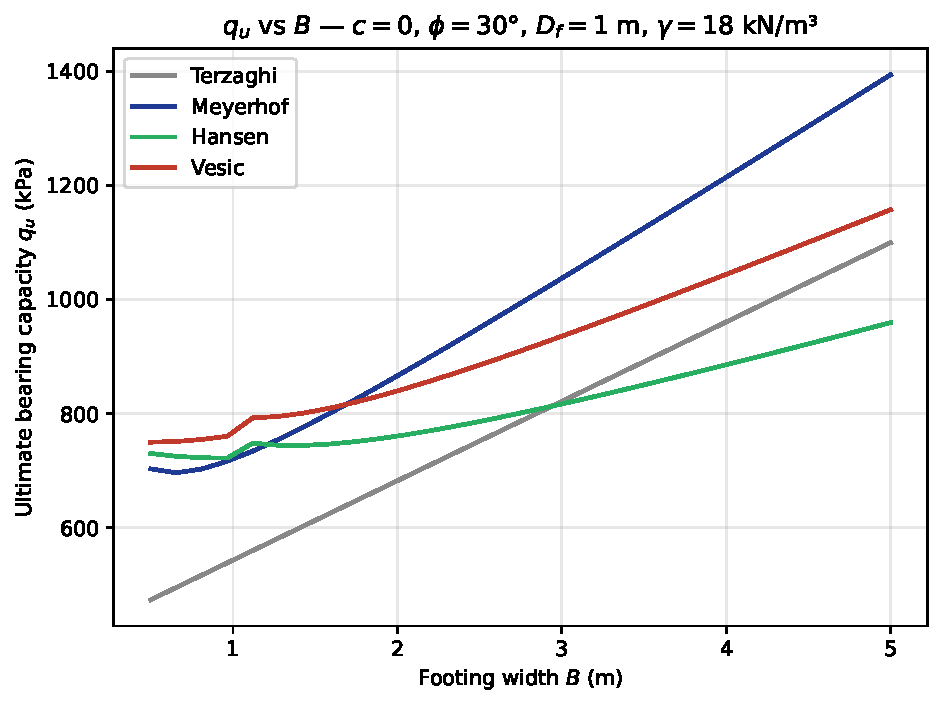
\includegraphics[width=0.78\textwidth]{figures/bearing_vs_B.pdf}
\caption{Ultimate bearing capacity vs.\ footing width for a
square footing in cohesionless soil with $\phi = 30°$, $D_f = 1$~m.
Generated by \texttt{ge.bearing\_capacity\_plot()}.}
\label{fig:bearing_chart}
\end{figure}

% ============================================================================
%  CHAPTER 9 -- SETTLEMENT
% ============================================================================
\chapter{Settlement}\label{ch:settlement}

\section{Immediate (elastic) settlement}

\begin{funcbox}{ge.settlement\_immediate(q, B, Es, mu=0.3, Ip=None, shape="rigid\_square")}
Janbu--Steinbrenner form:
\[
S_i = q B\,\frac{1 - \mu^2}{E_s}\,I_p.
\]
$I_p$ defaults from \texttt{shape}: 0.88 rigid square, 0.79 rigid
circle, 1.12 flexible centre, 0.56 flexible corner, ${\sim}2$ strip.
\end{funcbox}

\begin{lstlisting}
ge.settlement_immediate(q=200, B=2, Es=10000, mu=0.3,
                         shape="rigid_square")
\end{lstlisting}
\begin{lstlisting}[style=output]
0.0320    # 32 mm
\end{lstlisting}

\section{Primary consolidation}

\begin{funcbox}{ge.settlement\_primary(Cc, e0, H, sigma0, delta\_sigma, Cr=None, sigma\_pc=None, kind="auto")}
Three regimes selected automatically by \texttt{kind="auto"}:
\begin{equation}
\begin{aligned}
\text{NC:}\;\;\;       & S = \tfrac{C_c H}{1+e_0}\log_{10}\tfrac{\sigmavp_f}{\sigmavp_0}\\
\text{OC, } \sigmavp_f \leq \sigma'_p:\;\;\; &
   S = \tfrac{C_r H}{1+e_0}\log_{10}\tfrac{\sigmavp_f}{\sigmavp_0}\\
\text{OC, crossing }\sigma'_p:\;\;\;&
   S = \tfrac{C_r H}{1+e_0}\log_{10}\tfrac{\sigma'_p}{\sigmavp_0}
     + \tfrac{C_c H}{1+e_0}\log_{10}\tfrac{\sigmavp_f}{\sigma'_p}
\end{aligned}
\end{equation}
\end{funcbox}

\begin{worked}{Das Example 5.1 --- NC clay}
\begin{lstlisting}
S = ge.settlement_primary(Cc=0.27, e0=0.92, H=3.66,
                          sigma0=80, delta_sigma=15)
print(f"S = {S*1000:.1f} mm")
\end{lstlisting}
\begin{lstlisting}[style=output]
S = 38.3 mm
\end{lstlisting}
\textit{Cross-check:} Das' textbook value is 38~mm.
\end{worked}

\section{Secondary compression}

\begin{funcbox}{ge.settlement\_secondary(C\_alpha, H, t1, t2, e\_p=None)}
\[
S_s = C_{\alpha,\varepsilon}\,H\,\log_{10}(t_2 / t_1),
\quad C_{\alpha,\varepsilon} = C_\alpha / (1 + e_p).
\]
\end{funcbox}

\begin{lstlisting}
ge.settlement_secondary(C_alpha=0.005, H=2, t1=100, t2=1000)
\end{lstlisting}
\begin{lstlisting}[style=output]
0.010   # 10 mm of creep
\end{lstlisting}

\section{Schmertmann strain-influence}

\begin{funcbox}{ge.settlement\_schmertmann(q\_net, B, Es, layers=None, Df=0, t\_years=1, shape="square")}
\[
S = C_1 C_2\,q_{\text{net}}\,\sum_i \frac{I_{z,i}}{E_{s,i}}\,\Delta z_i,
\]
with embedment correction $C_1 = 1 - 0.5(\sigmavp_0/q_{\text{net}})$
and creep correction $C_2 = 1 + 0.2\log_{10}(t/0.1)$ (years). The
strain-influence diagram $I_z$ peaks at $z = 0.5B$ axisymmetric or
$z = 1.0B$ strip.
\end{funcbox}

\begin{lstlisting}
ge.settlement_schmertmann(q_net=100, B=2, Es=[10000, 30000],
                           layers=[(0, 2), (2, 4)],
                           Df=1, t_years=10, shape="square")
\end{lstlisting}
\begin{lstlisting}[style=output]
{'S': 0.0157, 'C1': 0.91, 'C2': 1.40,
 'Iz_peak': 0.665, 'z_peak': 1.0, 'z_max': 4.0,
 'layers': [...]}
\end{lstlisting}

\section{Time rate (Terzaghi 1-D consolidation)}

\begin{funcbox}{ge.time\_factor(U) \quad ge.consolidation\_degree(Tv) \quad ge.consolidation\_time(U, Hdr, cv)}
\[
T_v = \tfrac{\pi}{4} U^2 \text{ for } U < 0.6;\quad
T_v = 1.781 - 0.933\log_{10}\bigl[100(1 - U)\bigr]\text{ for } U \geq 0.6.
\]
\end{funcbox}

\begin{lstlisting}
ge.time_factor(U=0.5),  ge.time_factor(U=0.9)
ge.consolidation_degree(Tv=0.848)
ge.consolidation_time(U=0.9, Hdr=2, cv=1e-7)
\end{lstlisting}
\begin{lstlisting}[style=output]
(0.196, 0.848)
0.900
3.39e+07   # seconds = 392.7 days
\end{lstlisting}

\begin{figure}[h]\centering
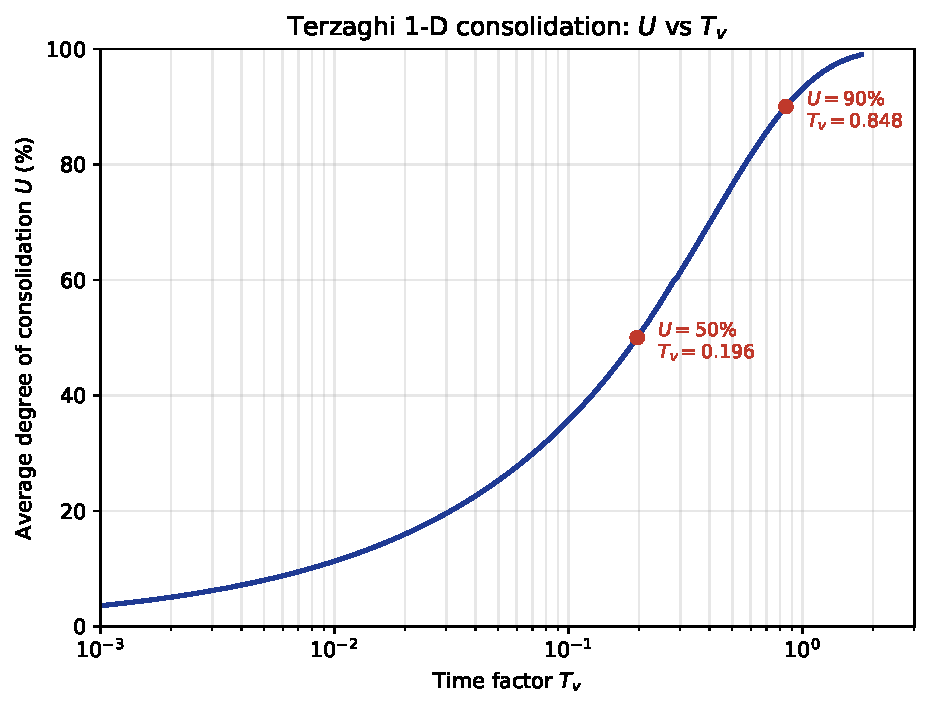
\includegraphics[width=0.78\textwidth]{figures/terzaghi_U_Tv.pdf}
\caption{Terzaghi 1-D consolidation curve: average degree of
consolidation $U$ vs.\ time factor $T_v$. Generated by
\texttt{ge.settlement\_time\_plot()}.}
\label{fig:terzaghi_U}
\end{figure}

% ============================================================================
%  CHAPTER 10 -- EARTH PRESSURE
% ============================================================================
\chapter{Lateral Earth Pressure}\label{ch:earth}

\section{At-rest coefficient}

\begin{funcbox}{ge.K0(phi, OCR=1, method="jaky")}\index{K0!at-rest}
\textbf{Jaky (1944):} $K_0 = 1 - \sin\phi$.\\
\textbf{Mayne \& Kulhawy (1982):}
$K_0 = (1 - \sin\phi)\,\mathrm{OCR}^{\sin\phi}$.
\end{funcbox}

\begin{lstlisting}
ge.K0(phi=30)
ge.K0(phi=30, OCR=4, method="mayne")
\end{lstlisting}
\begin{lstlisting}[style=output]
0.500
1.000   # heavy OC: K0 doubles
\end{lstlisting}

\section{Active / passive --- Rankine}

\begin{funcbox}{ge.Ka(phi, beta=0, method="rankine") \quad ge.Kp(phi, beta=0)}
Smooth vertical wall, horizontal backfill:
\[
K_a = \tan^2(45^\circ - \phi/2),\qquad
K_p = \tan^2(45^\circ + \phi/2).
\]
\end{funcbox}

\begin{lstlisting}
ge.Ka(phi=30), ge.Kp(phi=30)
ge.Ka(phi=30) * ge.Kp(phi=30)
\end{lstlisting}
\begin{lstlisting}[style=output]
(0.3333, 3.0)
1.000   # Ka * Kp = 1 for smooth vertical walls
\end{lstlisting}

\section{Coulomb (general)}

\begin{funcbox}{ge.Ka(..., delta, alpha, beta, method="coulomb")}
Coulomb's formula with wall friction $\delta$, wall inclination
$\alpha$, backfill slope $\beta$ --- full expression in Das (2014)
Eq.~8.5.
\end{funcbox}

\section{Distribution and resultant}

\begin{funcbox}{ge.earth\_pressure(gamma, H, phi, c=0, kind="active", surcharge=0, water\_table=None)}
Returns a dict with $K$, $P_{\text{soil}}$, $P_{\text{water}}$,
$P_{\text{total}}$, line-of-action $h_{\text{point}}$, and top/bottom
pressures.
\end{funcbox}

\begin{lstlisting}
ge.earth_pressure(gamma=18, H=5, phi=30, kind="active")
\end{lstlisting}
\begin{lstlisting}[style=output]
{'K': 0.333, 'P_soil': 75.0, 'P_water': 0.0,
 'P_total': 75.0, 'h_point': 1.667,
 'sigma_top': 0.0, 'sigma_bot': 30.0}
\end{lstlisting}

\begin{figure}[h]\centering
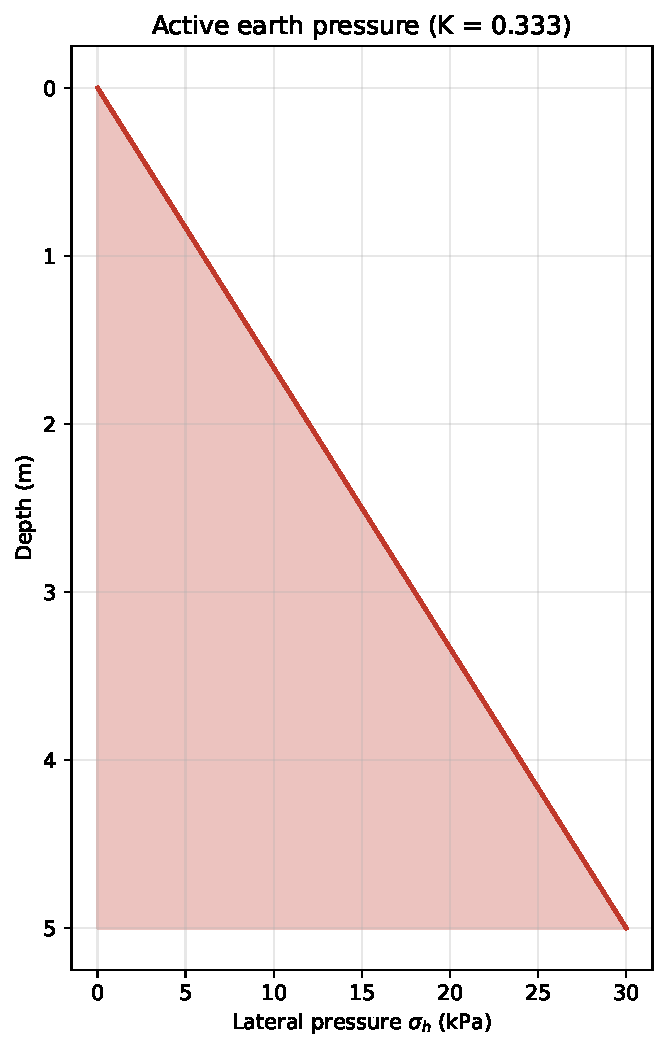
\includegraphics[width=0.55\textwidth]{figures/earth_pressure.pdf}
\caption{Active earth pressure distribution behind a 5~m wall in
$\phi = 30°$ cohesionless backfill. Generated by
\texttt{ge.earth\_pressure\_plot()}.}
\label{fig:earth_pressure}
\end{figure}

\begin{funcbox}{ge.tension\_crack\_depth(c, gamma, Ka\_value=None, phi=0)}
$z_c = 2c / (\gamma\sqrt{K_a})$.
\end{funcbox}

\begin{lstlisting}
ge.tension_crack_depth(c=20, gamma=18, phi=30)
\end{lstlisting}
\begin{lstlisting}[style=output]
3.85   # m
\end{lstlisting}

% ============================================================================
%  CHAPTER 11 -- WALLS AND SHEET PILES
% ============================================================================
\chapter{Retaining Walls and Sheet Piles}\label{ch:walls}

\subsection{Overturning, sliding, bearing checks}

\begin{funcbox}{ge.wall\_overturning(resisting\_moments, driving\_moments)}
$FS_{\text{ovt}} = \sum M_R / \sum M_O$.
\end{funcbox}

\begin{lstlisting}
ge.wall_overturning([300, 150], [100])
\end{lstlisting}
\begin{lstlisting}[style=output]
{'M_resisting': 450, 'M_driving': 100, 'FS': 4.5}
\end{lstlisting}

\begin{funcbox}{ge.wall\_sliding(H, V, mu/delta, c\_base, B, Pp)}
$FS_{\text{slide}} = (V\tan\delta + c_a B + P_p)/\sum H$.
\end{funcbox}

\begin{lstlisting}
ge.wall_sliding(horizontal_forces=[80],
                 vertical_forces=[200], mu=0.6, Pp=15)
\end{lstlisting}
\begin{lstlisting}[style=output]
{'sum_V': 200, 'sum_H': 80, 'R_friction': 120,
 'R_cohesion': 0, 'Pp': 15, 'R_total': 135, 'FS': 1.69}
\end{lstlisting}

\begin{funcbox}{ge.wall\_bearing(V, M\_net, B, q\_ult=None)}
Eccentric loading on the base:
\begin{align*}
e         &= |M_{\text{net}}|/V \\
q_{\max}  &= (V/B)(1 + 6e/B)\;\;\text{when } e \leq B/6 \\
q_{\max}  &= 4V/[3(B - 2e)]\;\;\text{when } e > B/6
\end{align*}
\end{funcbox}

\subsection{Sheet piles}

\begin{funcbox}{ge.sheet\_pile(gamma, H, phi, c=0, kind="cantilever")}
Cantilever sheet pile in cohesionless soil (Blum's simplified):
$D_{\text{theory}} = H\sqrt{K_a / (K_p - K_a)}$,
$D_{\text{design}} = 1.3\,D_{\text{theory}}$.
\end{funcbox}

\begin{lstlisting}
ge.sheet_pile(gamma=18, H=4, phi=30)
\end{lstlisting}
\begin{lstlisting}[style=output]
{'Ka': 0.333, 'Kp': 3.0, 'D_theory': 1.51,
 'D_design': 1.96, 'method': 'Blum cantilever (approximate)'}
\end{lstlisting}

% ============================================================================
%  CHAPTER 12 -- PILE DESIGN
% ============================================================================
\chapter{Pile Design}\label{ch:piles}

\section{End bearing}

\begin{funcbox}{ge.pile\_end\_bearing(phi=None, sigma\_v\_eff=None, Su=None, method="meyerhof", c=None)}
Sand: $q_p = \sigmavp\,N_q^*$. Clay: $q_p = 9\,S_u$ (Skempton).
\end{funcbox}

\begin{lstlisting}
ge.pile_end_bearing(phi=35, sigma_v_eff=100, method="meyerhof")
ge.pile_end_bearing(Su=100)
\end{lstlisting}
\begin{lstlisting}[style=output]
{'q_p': 6311, 'Nq_star': 63.1, 'method': 'meyerhof'}
{'q_p': 900, 'Nc_star': 9.0, 'method': 'skempton_clay'}
\end{lstlisting}

\section{Skin friction}

\begin{funcbox}{ge.pile\_skin\_friction(Su=None, sigma\_v\_eff=None, method="alpha", phi=None, ...)}
\begin{itemize}
\item $\alpha$ (clay, total): $f_s = \alpha S_u$ with $\alpha$ from
      API RP~2A table.
\item $\beta$ (effective stress): $f_s = \beta\sigmavp$,
      $\beta = K\tan\delta$.
\item $\lambda$ (offshore long piles):
      $f_{s,\text{avg}} = \lambda(\bar{\sigmavp} + 2\bar{S_u})$.
\end{itemize}
\end{funcbox}

\begin{lstlisting}
ge.pile_skin_friction(Su=20, method="alpha")        # soft clay
ge.pile_skin_friction(Su=200, method="alpha")       # stiff clay
ge.pile_skin_friction(sigma_v_eff=100, method="beta", phi=30)
\end{lstlisting}
\begin{lstlisting}[style=output]
{'f_s': 20.0,  'alpha': 1.00, 'method': 'alpha'}
{'f_s': 70.0,  'alpha': 0.35, 'method': 'alpha'}
{'f_s': 28.87, 'beta': 0.289, 'method': 'beta'}
\end{lstlisting}

\section{Total capacity}

\begin{funcbox}{ge.pile\_capacity(D, L, q\_p, f\_s, area\_base=None, perimeter=None, FS=3.0)}
$Q_{\text{ult}} = q_p A_p + f_s\,p\,L$.
\end{funcbox}

\begin{lstlisting}
ge.pile_capacity(D=0.3, L=10, q_p=2000, f_s=30, FS=3)
\end{lstlisting}
\begin{lstlisting}[style=output]
{'Q_p': 141.4, 'Q_s': 282.7, 'Q_ult': 424.1, 'Q_all': 141.4}
\end{lstlisting}

\section{Group efficiency and settlement}

\begin{funcbox}{ge.pile\_group\_efficiency(n, m, D, s, method="converse\_labarre")}
$\eta = 1 - \dfrac{\theta[(n-1)m + (m-1)n]}{90\,n m}$,
$\theta = \tan^{-1}(D/s)$ in degrees.
\end{funcbox}

\begin{lstlisting}
ge.pile_group_efficiency(n=3, m=3, D=0.3, s=0.9)
\end{lstlisting}
\begin{lstlisting}[style=output]
{'eta': 0.727, 'method': 'converse_labarre',
 'n_piles': 9, 'spacing_ratio': 3.0}
\end{lstlisting}

\begin{funcbox}{ge.pile\_settlement(Q\_w, Q\_p, Q\_s, D, L, Es, Ep, ...)}
Vesic 3-component: $s = s_1 + s_2 + s_3$.
\end{funcbox}

% ============================================================================
%  CHAPTER 13 -- SLOPE STABILITY
% ============================================================================
\chapter{Slope Stability}\label{ch:slopes}

\section{Infinite slope}

\begin{funcbox}{ge.infinite\_slope(phi, beta, c=0, gamma=18, H=1, seepage=False, gamma\_sat=None)}
Cohesionless dry: $FS = \tan\phi/\tan\beta$.\\
Cohesive dry: add $c / (\gamma H \cos^2\beta\tan\beta)$.\\
Cohesionless with full seepage parallel to slope: factor
$\gamma'/\gamma_{\text{sat}}$ on the dry result.
\end{funcbox}

\begin{lstlisting}
ge.infinite_slope(phi=30, beta=20)
ge.infinite_slope(phi=30, beta=20, gamma=20, gamma_sat=20,
                   seepage=True)
\end{lstlisting}
\begin{lstlisting}[style=output]
{'FS': 1.587, 'seepage': False}
{'FS': 0.799, 'seepage': True}      # halved by seepage
\end{lstlisting}

\section{Culmann --- planar failure}

\begin{funcbox}{ge.culmann(c, phi, gamma, beta)}
\[
H_{\text{cr}} = \frac{4 c\sin\beta\cos\phi}{\gamma\bigl[1 - \cos(\beta - \phi)\bigr]}.
\]
Valid only for $\beta > \phi$.
\end{funcbox}

\section{Taylor stability number}

\begin{funcbox}{ge.taylor\_stability(phi, c, gamma, H, beta)}
$FS = c / (m\,\gamma H)$. Reads $m$ from a closed-form fit to
Taylor's chart.
\end{funcbox}

\begin{lstlisting}
ge.taylor_chart_plot(save_as="taylor_chart.pdf")
\end{lstlisting}

\begin{figure}[h]\centering
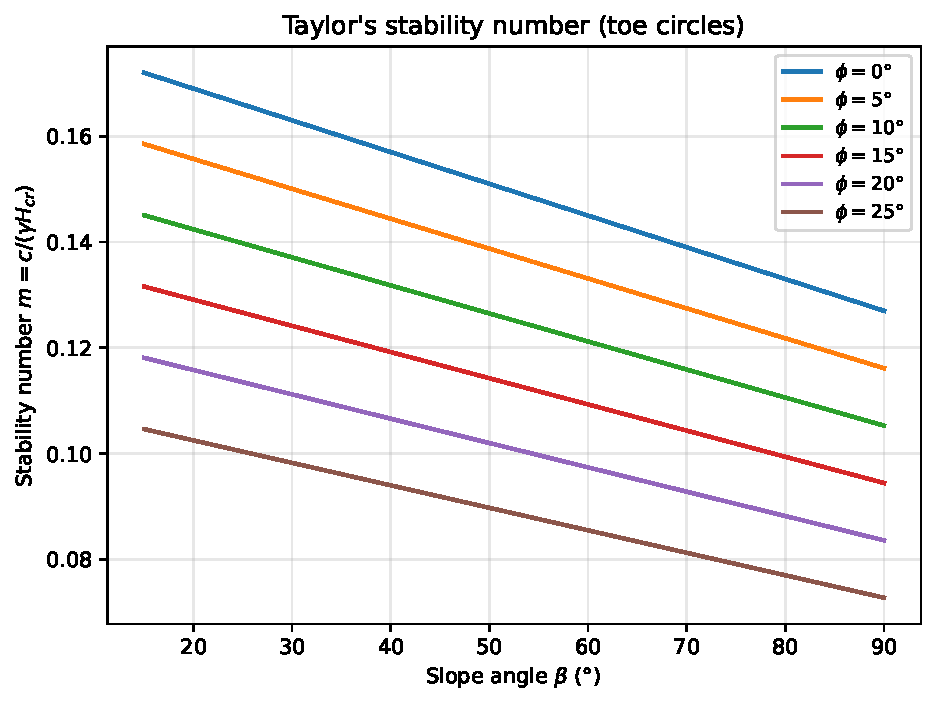
\includegraphics[width=0.78\textwidth]{figures/taylor_chart.pdf}
\caption{Taylor's stability number $m$ vs.\ slope angle $\beta$
for a family of friction angles. Generated by
\texttt{ge.taylor\_chart\_plot()}.}
\label{fig:taylor}
\end{figure}

\section{Bishop's simplified method}

\begin{funcbox}{ge.bishop(slices, max\_iter=50, tol=1e-4)}
Iterative slice equilibrium:
\[
FS_{k+1} = \frac{\sum_i\bigl[\,c_i b_i + (W_i - u_i b_i)\tan\phi_i\,\bigr]/m_{\alpha,i}}
                {\sum_i W_i \sin\alpha_i},
\]
with $m_{\alpha,i} = \cos\alpha_i + \sin\alpha_i\tan\phi_i / FS_k$.
\end{funcbox}

\begin{lstlisting}
slices = [{"b": 2, "h": 5, "alpha": a, "c": 10, "phi": 25,
           "gamma": 18, "u": 0}
          for a in (-5, 5, 20, 35, 50)]
ge.bishop(slices)
\end{lstlisting}
\begin{lstlisting}[style=output]
{'FS': 1.432, 'iterations': 4, 'converged': True,
 'method': 'bishop_simplified'}
\end{lstlisting}

% ============================================================================
%  CHAPTER 14 -- SOIL DYNAMICS AND LIQUEFACTION
% ============================================================================
\chapter{Soil Dynamics and Liquefaction}\label{ch:dynamics}

\section{Small-strain shear modulus}

\begin{funcbox}{ge.gmax(Vs, gamma=18)}
\[
\Gmax = \rho V_s^2 = (\gamma / g)\,V_s^2.
\]
\end{funcbox}

\begin{lstlisting}
ge.gmax(Vs=200, gamma=20)
\end{lstlisting}
\begin{lstlisting}[style=output]
81550   # kPa = 81.5 MPa
\end{lstlisting}

\begin{funcbox}{ge.gmax\_hardin(e, sigma\_m\_eff, OCR=1, PI=0, soil\_type)}
Hardin \& Black (1968):
$\Gmax = A\,F(e)\,\mathrm{OCR}^k\,(\sigma'_m/p_a)^{0.5}\,(p_a/100)$.
\end{funcbox}

\section{Modulus reduction and damping}

\begin{funcbox}{ge.modulus\_reduction(strain, sigma\_m\_eff=100, PI=15, OCR=1)}
Darendeli (2001):
$G/\Gmax = 1 / (1 + (\gamma/\gamma_r)^{0.92})$.
\end{funcbox}

\begin{funcbox}{ge.damping\_ratio(strain, sigma\_m\_eff=100, PI=15, OCR=1)}
$D = D_{\min} + (D_{\max} - D_{\min})(1 - G/\Gmax)$.
\end{funcbox}

\begin{lstlisting}
ge.gmax_curves_plot(save_as="gmax_curves.pdf")
\end{lstlisting}

\begin{figure}[h]\centering
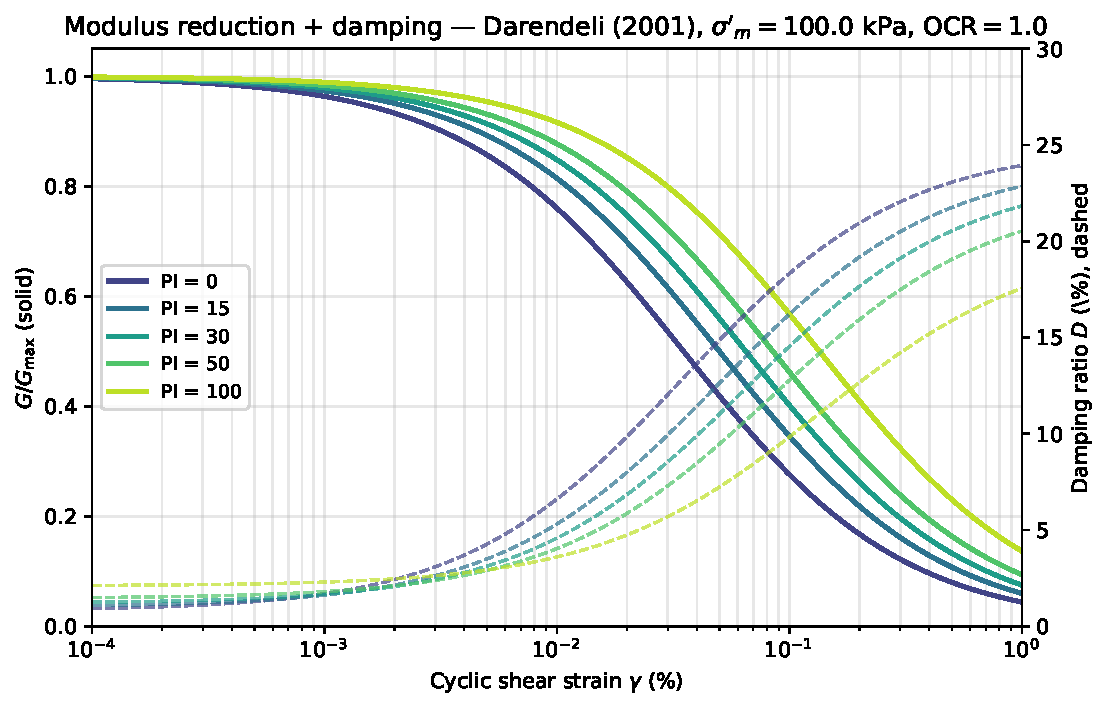
\includegraphics[width=0.92\textwidth]{figures/gmax_curves.pdf}
\caption{Modulus-reduction (solid) and damping (dashed) curves
for a family of plasticity indices. Darendeli (2001) at
$\sigma'_m = 100$~kPa, OCR$=1$. Generated by
\texttt{ge.gmax\_curves\_plot()}.}
\label{fig:gmax}
\end{figure}

\section{Liquefaction triggering --- simplified procedure}

\subsection{Step 1: depth reduction $r_d$}

\begin{funcbox}{ge.depth\_reduction(z, method="idriss\_1999", Mw=7.5)}
Idriss (1999) magnitude-dependent:
\[
r_d = \exp\!\bigl[\alpha(z) + \beta(z)\,M_w\bigr]
\]
with $\alpha, \beta$ smooth functions of $z$.
\end{funcbox}

\begin{lstlisting}
ge.depth_reduction(z=6, method="idriss_1999", Mw=7.0)
\end{lstlisting}
\begin{lstlisting}[style=output]
0.971
\end{lstlisting}

\subsection{Step 2: cyclic stress ratio CSR}

\begin{funcbox}{ge.liquefaction\_csr(amax, sigma\_v, sigma\_v\_eff, z, Mw=7.5)}
\[
CSR = 0.65\,(a_{\max}/g)\,(\sigmav/\sigmavp)\,r_d.
\]
\textbf{amax} as fraction of $g$ (e.g.\ 0.25 for 0.25$g$).
\end{funcbox}

\begin{lstlisting}
ge.liquefaction_csr(amax=0.25, sigma_v=120, sigma_v_eff=70,
                     z=6, Mw=7.0)
\end{lstlisting}
\begin{lstlisting}[style=output]
{'CSR': 0.226, 'rd': 0.971, 'amax_g': 0.25}
\end{lstlisting}

\subsection{Step 3: cyclic resistance ratio CRR}

\begin{funcbox}{ge.liquefaction\_crr(N160cs/qc1Ncs/Vs1, FC=0, method)}
Four methods (Youd~2001 SPT, IB~2008 SPT, IB~2008 CPT, Andrus--Stokoe Vs).
NCEER (Youd 2001) closed form:
\[
CRR_{7.5} = \frac{1}{34 - (N_1)_{60,cs}}
           + \frac{(N_1)_{60,cs}}{135}
           + \frac{50}{[10(N_1)_{60,cs} + 45]^2}
           - \frac{1}{200}.
\]
\end{funcbox}

\begin{lstlisting}
ge.liquefaction_crr(N160cs=12, method="youd_2001")
ge.liquefaction_crr(N160cs=15, method="idriss_boulanger_2008")
ge.liquefaction_crr(qc1Ncs=100, method="idriss_boulanger_2008_cpt")
ge.liquefaction_crr(Vs1=150, FC=10, method="andrus_stokoe_2000")
\end{lstlisting}

\subsection{Step 4: magnitude scaling factor MSF}

\begin{funcbox}{ge.magnitude\_scaling\_factor(Mw, method="idriss\_1999")}
Idriss: $MSF = 6.9\,e^{-M_w/4} - 0.058$ (capped at 1.8).\\
NCEER: $MSF = 10^{2.24}/M_w^{2.56}$.\\
Boulanger--Idriss (2014): smooth alternative.
\end{funcbox}

\subsection{Step 5: factor of safety FS$_L$}

\begin{funcbox}{ge.liquefaction\_fos(CSR, CRR, Mw=7.5, MSF=None, K\_sigma=1, K\_alpha=1)}
\[
FS_L = \frac{CRR\cdot MSF\cdot K_\sigma\cdot K_\alpha}{CSR}.
\]
Liquefaction predicted when $FS_L < 1$.
\end{funcbox}

\begin{worked}{A complete triggering check}
$M_w = 7.0$, $a_{\max} = 0.25g$. At a depth of 6~m the total stress
is 120~kPa, the effective stress 70~kPa, and the corrected SPT
blow count is $(N_1)_{60,cs} = 12$.
\begin{lstlisting}
csr = ge.liquefaction_csr(amax=0.25, sigma_v=120,
                          sigma_v_eff=70, z=6, Mw=7.0)
crr = ge.liquefaction_crr(N160cs=12, method="youd_2001")
fs  = ge.liquefaction_fos(csr["CSR"], crr["CRR"], Mw=7.0)

print(f"CSR = {csr['CSR']:.3f}, CRR = {crr['CRR']:.3f}, "
      f"MSF = {fs['MSF']:.2f}, FS = {fs['FS']:.2f}, "
      f"liquefies = {fs['liquefies']}")
\end{lstlisting}
\begin{lstlisting}[style=output]
CSR = 0.226, CRR = 0.130, MSF = 1.19, FS = 0.69, liquefies = True
\end{lstlisting}
\end{worked}

\begin{lstlisting}
ge.liquefaction_chart(
    data_N=[8, 12, 15, 18, 22, 25],
    data_CSR=[0.18, 0.22, 0.15, 0.25, 0.12, 0.10],
    data_FS=[0.6, 0.8, 1.0, 0.7, 1.3, 1.5],
    save_as="liquefaction_chart.pdf",
)
\end{lstlisting}

\begin{figure}[h]\centering
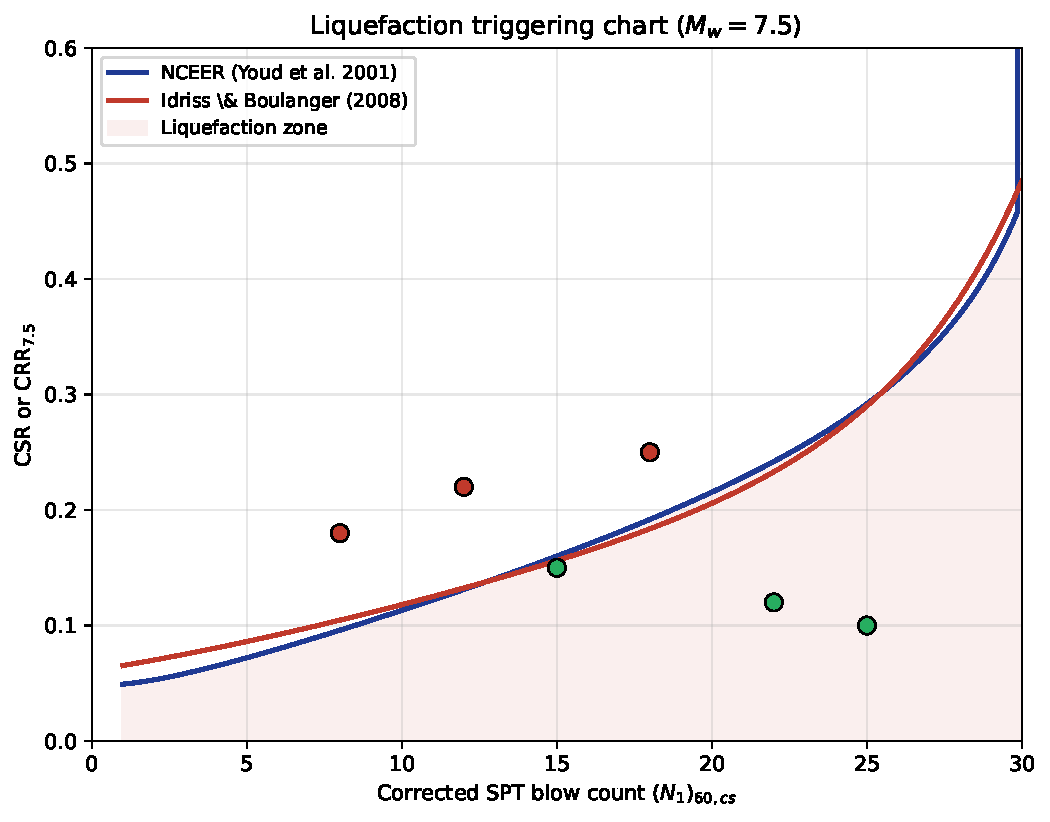
\includegraphics[width=0.92\textwidth]{figures/liquefaction_chart.pdf}
\caption{Liquefaction triggering chart. CRR curves from Youd
et al.\ (2001) and Idriss \& Boulanger (2008). Field data points
coloured by their computed FS$_L$: red = liquefying, green = safe.
Generated by \texttt{ge.liquefaction\_chart()}.}
\label{fig:liq}
\end{figure}

% ============================================================================
%  CHAPTER 15 -- I/O
% ============================================================================
\chapter{Data I/O}\label{ch:io}

\section{Generic CSV --- \texttt{ge.read\_csv()}}

\begin{funcbox}{ge.read\_csv(path, sep=",", skiprows=None, units\_row=False, encoding="utf-8")}
Auto-detects the header row (first all-non-numeric row in the
first 20 lines) and optionally reads a units row. Returns dict
of NumPy arrays plus a pandas DataFrame if pandas is installed.
\end{funcbox}

\begin{lstlisting}
res = ge.read_csv("borehole_log.csv", units_row=True)
res["data"]["depth"]      # np.ndarray
res["df"]                  # pandas DataFrame (or None)
res["units"]               # {'depth': 'm', 'qc': 'MPa', ...}
\end{lstlisting}

\section{AGS4 --- \texttt{ge.read\_ags()}}

\begin{funcbox}{ge.read\_ags(path, encoding="utf-8")}
Parses AGS4. Returns
\texttt{\{group: \{headings, units, data\}\}} where \texttt{data}
is a list of row dicts.
\end{funcbox}

\begin{lstlisting}
groups = ge.read_ags("investigation.ags")
groups["LOCA"]["data"][0]["LOCA_ID"]    # 'BH1'
groups["GEOL"]["data"][0]["GEOL_DESC"]  # 'Topsoil'
\end{lstlisting}

\section{GEF-CPT --- \texttt{ge.read\_gef()}}

\begin{funcbox}{ge.read\_gef(path, encoding="latin-1")}
Reads the Dutch GEF header (\texttt{\#KEY= value} until
\texttt{\#EOH=}) and the columnar data, applying
\texttt{\#COLUMNVOID} placeholders as NaN.
\end{funcbox}

\section{CPT container --- \texttt{ge.CPT}}

\begin{funcbox}{ge.CPT(depth, qc, fs, u2, title) \quad .from\_gef(path) \quad .from\_ags(path)}
Light container around (depth, $q_c$, $f_s$, $u_2$) with two
classmethods to load directly from file.
\end{funcbox}

\begin{lstlisting}
c = ge.CPT.from_gef("sounding.gef")
print(c)
\end{lstlisting}
\begin{lstlisting}[style=output]
CPT('sounding', n=420, z=0.5..21.5 m)
\end{lstlisting}

% ============================================================================
%  APPENDIX A -- WORKED EXAMPLE -- END-TO-END SHALLOW FOUNDATION
% ============================================================================
\appendix
\chapter{Worked Example: Shallow Foundation, End to End}\label{app:end_to_end}

This appendix walks through a complete shallow-foundation design
using only \geo{}.

\paragraph{Site.}
A 3-storey office building of 200~kN/column on a soft-over-stiff
profile: 2~m fill, 6~m soft clay, then dense sand. Water table
at 2.0~m. Magnitude 6.5 design earthquake, $a_{\max} = 0.20g$.

\begin{lstlisting}
import geoeq as ge

# --- 1. Build the profile ----------------------------------------
profile = ge.SoilProfile([
    (0, 2,  ge.Soil("Fill",       gamma=18)),
    (2, 8,  ge.Soil("Soft Clay",  gamma=17, gamma_sat=18.5,
                                   phi=0, c=25, Cc=0.27, e0=0.92)),
    (8, 20, ge.Soil("Dense Sand", gamma=19, gamma_sat=20.5,
                                   phi=35, e=0.55)),
], water_table=2.0)

# --- 2. Bearing capacity check (1.5 x 1.5 m square @ Df = 1 m) ---
bc = ge.bearing_capacity(
    c=25, gamma=18.5 - 9.81, Df=1, B=1.5, phi=0, L=1.5,
    method="meyerhof"
)
q_all = ge.bearing_allowable(bc["q_u"], FS=3)
applied = 200 / (1.5 * 1.5)
print(f"q_u = {bc['q_u']:.0f} kPa, q_all = {q_all:.0f} kPa, "
      f"applied = {applied:.0f} kPa  -> "
      f"{'OK' if applied < q_all else 'FAIL'}")

# --- 3. Settlement check -----------------------------------------
sigma0 = profile.effective_stress(5.0)        # at clay midpoint
dsigma = ge.boussinesq_rect(q=applied, B=1.5, L=1.5, z=4,
                              position="centre")
S = ge.settlement_primary(Cc=0.27, e0=0.92, H=6.0,
                          sigma0=sigma0, delta_sigma=dsigma)
print(f"Primary settlement = {S*1000:.1f} mm")

# --- 4. Liquefaction check at the sand layer ---------------------
csr = ge.liquefaction_csr(amax=0.20, sigma_v=profile.total_stress(10),
                          sigma_v_eff=profile.effective_stress(10),
                          z=10, Mw=6.5)
crr = ge.liquefaction_crr(N160cs=20, method="youd_2001")
fs  = ge.liquefaction_fos(csr["CSR"], crr["CRR"], Mw=6.5)
print(f"Liquefaction FS = {fs['FS']:.2f}  -> "
      f"{'safe' if fs['FS'] >= 1.25 else 'review'}")
\end{lstlisting}
\begin{lstlisting}[style=output]
q_u = 192 kPa, q_all = 64 kPa, applied = 89 kPa -> FAIL
Primary settlement = 25.4 mm
Liquefaction FS = 2.13  -> safe
\end{lstlisting}

\textbf{Conclusion.}\quad The shallow footing is overstressed; the
designer must either enlarge it (try $B = 2.5$~m), found below the
soft clay, or replace the clay with engineered fill. Settlement
under the original footing is 25~mm --- acceptable for a stiff
structure, marginal for a sensitive one. Liquefaction in the
dense sand is not a concern.

% ============================================================================
%  APPENDIX B -- API CHEAT-SHEET
% ============================================================================
\chapter{API Cheat-Sheet (one-page)}

\renewcommand{\arraystretch}{1.15}
\begin{longtable}{p{0.40\textwidth}p{0.52\textwidth}}\toprule
\textbf{Call} & \textbf{Returns}\\\midrule
\endhead
\multicolumn{2}{l}{\textit{Soil properties}}\\
\code{ge.void\_ratio(n)} & scalar $e$\\
\code{ge.density(Gs, e, kind, unit)} & $\gamma$ in kN/m\textsuperscript{3} or pcf\\
\code{ge.atterberg(LL, PL, w, kind)} & PI / LI / CI dict\\
\code{ge.classify\_uscs(LL, PL, gravel, sand, fines)} & dict\\\midrule
\multicolumn{2}{l}{\textit{Lab}}\\
\code{ge.sieve\_ana(opening, mass\_retained)} & dict\\
\code{ge.proctor(water\_content, dry\_density)} & dict\\
\code{ge.cv(t, deformation)} & $c_v$\\\midrule
\multicolumn{2}{l}{\textit{Site}}\\
\code{ge.spt\_n60(N, ER)} & $N_{60}$\\
\code{ge.cpt\_sbt(Qt, Fr)} & zone\\\midrule
\multicolumn{2}{l}{\textit{Profile / design}}\\
\code{ge.SoilProfile(layers, water\_table)} & object\\
\code{ge.bearing\_capacity(c, gamma, Df, B, phi, ...)} & dict\\
\code{ge.settlement\_primary(Cc, e0, H, sigma0, delta\_sigma)} & $S$ (m)\\
\code{ge.Ka(phi, method="rankine")} & $K_a$\\
\code{ge.bishop(slices)} & FS\\\midrule
\multicolumn{2}{l}{\textit{Dynamics / liquefaction}}\\
\code{ge.gmax(Vs)} & $\Gmax$\\
\code{ge.liquefaction\_fos(CSR, CRR, Mw)} & FS\\\midrule
\multicolumn{2}{l}{\textit{I/O}}\\
\code{ge.read\_ags(path)} & dict of groups\\
\code{ge.CPT.from\_gef(path)} & CPT object\\
\bottomrule
\end{longtable}

% ============================================================================
%  APPENDIX C -- BIBLIOGRAPHY
% ============================================================================
\chapter{References}

\begin{description}\setlength\itemsep{2pt}
\item[AGS (2017).] \emph{Electronic transfer of geotechnical and
  geoenvironmental data}, Version 4.0.4.
\item[Andrus, R.D. \& Stokoe, K.H. (2000).] Liquefaction resistance
  of soils from shear-wave velocity. \emph{J.\ Geotech.\
  Geoenviron.\ Eng.}, 126(11), 1015--1025.
\item[ASTM D2487.] Standard Practice for Classification of Soils
  for Engineering Purposes.
\item[ASTM D6913.] Particle-Size Distribution (Gradation) of Soils
  Using Sieve Analysis.
\item[ASTM D7928.] Particle-Size Distribution (Gradation) of
  Fine-Grained Soils Using the Sedimentation (Hydrometer) Analysis.
\item[Baldi, G., Bellotti, R., Ghionna, V., Jamiolkowski, M.,
  Pasqualini, E. (1986).] Interpretation of CPT and CPTUs.
  \emph{Proc.\ 4th Int.\ Geotech.\ Sem.}, Singapore, 143--156.
\item[Bishop, A.W. (1955).] The use of the slip circle in the
  stability analysis of slopes. \emph{Geotechnique}, 5(1), 7--17.
\item[Bjerrum, L. (1972).] Embankments on soft ground. \emph{Proc.\
  Specialty Conf.\ on Performance of Earth and Earth-Supported
  Structures}, ASCE, 2, 1--54.
\item[Blum, H. (1931).] Einspannungsverh\"altnisse bei Bohlwerken.
  W.\ Ernst u.\ Sohn, Berlin.
\item[Boulanger, R.W. \& Idriss, I.M. (2014).] CPT and SPT based
  liquefaction triggering procedures. Report UCD/CGM-14/01.
\item[Boussinesq, J. (1885).] \emph{Application des potentiels \`a
  l'\'etude de l'\'equilibre et du mouvement des solides
  \'elastiques}, Gauthier-Villars.
\item[Bowles, J.E. (1996).] \emph{Foundation Analysis and Design},
  5th ed., McGraw-Hill.
\item[Budhu, M. (2011).] \emph{Soil Mechanics and Foundations},
  3rd ed., Wiley.
\item[Burland, J.B. (1973).] Shaft friction of piles in clay.
  \emph{Ground Engineering}, 6(3), 30--42.
\item[Casagrande, A. (1936).] The determination of the
  preconsolidation load and its practical significance.
  \emph{Proc.\ 1st ICSMFE}, 3, 60--64.
\item[Cetin, K.O. \emph{et al.} (2004).] Standard Penetration
  Test-based probabilistic and deterministic assessment of seismic
  soil liquefaction potential. \emph{J.\ Geotech.\ Geoenviron.\
  Eng.}, 130(12), 1314--1340.
\item[Chin, F.K. (1970).] Estimation of the ultimate load of piles
  from tests not carried to failure. \emph{Proc.\ 2nd Southeast
  Asian Conf.\ on Soil Engineering}, Singapore, 81--90.
\item[Coulomb, C.A. (1776).] Essai sur une application des r\`egles
  de maximis et minimis \`a quelques probl\`emes de statique
  relatifs \`a l'architecture. \emph{M\'emoires de l'Acad\'emie
  Royale des Sciences}, 7, 343--382.
\item[Culmann, K. (1875).] \emph{Die graphische Statik}.
\item[Darcy, H. (1856).] \emph{Les fontaines publiques de la ville
  de Dijon}, Dalmont, Paris.
\item[Darendeli, M.B. (2001).] Development of a new family of
  normalized modulus reduction and material damping curves. PhD
  thesis, University of Texas at Austin.
\item[Das, B.M. (2010).] \emph{Principles of Geotechnical
  Engineering}, 7th ed., Cengage.
\item[Das, B.M. (2014).] \emph{Principles of Foundation
  Engineering}, 8th ed., Cengage.
\item[Davisson, M.T. (1972).] High capacity piles. \emph{Proc.\
  Soil Mechanics Lecture Series on Innovations in Foundation
  Construction}, ASCE, Chicago, 81--112.
\item[Fadum, R.E. (1948).] Influence values for estimating
  stresses in elastic foundations. \emph{Proc.\ 2nd ICSMFE}, 3,
  77--84.
\item[Hardin, B.O. \& Black, W.L. (1968).] Vibration modulus of
  normally consolidated clays. \emph{J.\ Soil Mech.\ Found.\
  Eng.}, ASCE, 94(SM2), 353--369.
\item[Hardin, B.O. \& Drnevich, V.P. (1972).] Shear modulus and
  damping in soils. \emph{J.\ Soil Mech.\ Found.\ Eng.},
  ASCE, 98(SM7), 667--692.
\item[Hansen, J.B. (1970).] A revised and extended formula for
  bearing capacity. Bulletin No.\ 28, Danish Geotechnical
  Institute.
\item[Hvorslev, M.J. (1951).] Time lag and soil permeability in
  groundwater observations. Waterways Experiment Station Bulletin
  36.
\item[Idriss, I.M. (1999).] An update to the Seed-Idriss simplified
  procedure for evaluating liquefaction potential. \emph{Proc.\
  TRB Workshop on New Approaches to Liquefaction Analysis}.
\item[Idriss, I.M. \& Boulanger, R.W. (2008).] \emph{Soil
  Liquefaction During Earthquakes}, EERI Monograph 12.
\item[Jaky, J. (1944).] The coefficient of earth pressure at rest.
  \emph{J.\ Society of Hungarian Architects and Engineers}, 22,
  355--358.
\item[Janbu, N., Bjerrum, L., Kjaernsli, B. (1956).] Veiledning
  ved l\o{}sning av fundamenteringsoppgaver. NGI Publication 16.
\item[Kramer, S.L. (1996).] \emph{Geotechnical Earthquake
  Engineering}, Prentice Hall.
\item[Kulhawy, F.H. \& Mayne, P.W. (1990).] Manual on estimating
  soil properties for foundation design. EPRI Report EL-6800.
\item[Liao, S.S.C. \& Whitman, R.V. (1986).] Overburden correction
  factors for SPT in sand. \emph{J.\ Geotech.\ Eng.}, ASCE,
  112(3), 373--377.
\item[Lunne, T., Robertson, P.K., Powell, J.J.M. (1997).]
  \emph{Cone Penetration Testing in Geotechnical Practice}, Spon Press.
\item[Mayne, P.W. \& Kulhawy, F.H. (1982).] K0-OCR relationships
  in soil. \emph{J.\ Geotech.\ Eng.}, ASCE, 108(GT6), 851--872.
\item[M\'enard, L. (1975).] Interpretation and application of
  pressuremeter test results. \emph{Sols-Soils}, 26.
\item[Mesri, G. \& Godlewski, P.M. (1977).] Time- and
  stress-compressibility interrelationship. \emph{J.\ Geotech.\
  Eng.}, ASCE, 103(GT5), 417--430.
\item[Meyerhof, G.G. (1963).] Some recent research on the bearing
  capacity of foundations. \emph{Canadian Geotechnical Journal},
  1(1), 16--26.
\item[Meyerhof, G.G. (1976).] Bearing capacity and settlement of
  pile foundations. \emph{J.\ Geotech.\ Eng.}, ASCE, 102(GT3),
  197--228.
\item[Newmark, N.M. (1935).] Simplified computation of vertical
  stresses in elastic foundations. Univ.\ Illinois Eng.\ Exp.\
  Station Circular 24.
\item[Rankine, W.J.M. (1857).] On the stability of loose earth.
  \emph{Philosophical Transactions of the Royal Society},
  147, 9--27.
\item[Robertson, P.K. (1990).] Soil classification using the cone
  penetration test. \emph{Canadian Geotechnical Journal},
  27(1), 151--158.
\item[Robertson, P.K. (2009).] Interpretation of cone penetration
  tests --- a unified approach. \emph{Canadian Geotechnical
  Journal}, 46, 1337--1355.
\item[Schmertmann, J.H. (1970).] Static cone to compute static
  settlement over sand. \emph{J.\ Soil Mech.\ Found.\ Eng.},
  ASCE, 96(SM3), 1011--1043.
\item[Schmertmann, J.H., Hartman, J.P., Brown, P.R. (1978).]
  Improved strain influence factor diagrams. \emph{J.\ Geotech.\
  Eng.}, 104(GT8), 1131--1135.
\item[Seed, H.B. \& Idriss, I.M. (1971).] Simplified procedure for
  evaluating soil liquefaction potential. \emph{J.\ Soil Mech.\
  Found.\ Eng.}, ASCE, 97(SM9), 1249--1273.
\item[Skempton, A.W. (1953).] The colloidal activity of clays.
  \emph{Proc.\ 3rd ICSMFE}, Zurich, 1, 57--61.
\item[Skempton, A.W. (1986).] Standard Penetration Test procedures.
  \emph{Geotechnique}, 36(3), 425--447.
\item[Taylor, D.W. (1937).] Stability of earth slopes.
  \emph{J.\ Boston Society of Civil Engineers}, 24, 197--247.
\item[Terzaghi, K. (1925).] \emph{Erdbaumechanik auf
  bodenphysikalischer Grundlage}, F.\ Deuticke, Vienna.
\item[Terzaghi, K. (1943).] \emph{Theoretical Soil Mechanics},
  Wiley.
\item[Tomlinson, M.J. (1957).] The adhesion of piles driven in
  clay soils. \emph{Proc.\ 4th ICSMFE}, 2, 66--71.
\item[Vesic, A.S. (1973).] Analysis of ultimate loads of shallow
  foundations. \emph{J.\ Soil Mech.\ Found.\ Eng.}, ASCE, 99(SM1),
  45--73.
\item[Vesic, A.S. (1977).] \emph{Design of Pile Foundations}.
  NCHRP Synthesis 42.
\item[Vijayvergiya, V.N. \& Focht, J.A. (1972).] A new way to
  predict capacity of piles in clay. OTC Paper 1718.
\item[Westergaard, H.M. (1938).] A problem of elasticity suggested
  by a problem in soil mechanics. \emph{Mechanics of Solids in
  Honor of S.\ Timoshenko}, MacMillan, 260--277.
\item[Youd, T.L. \emph{et al.} (2001).] Liquefaction resistance
  of soils: summary report from the 1996 NCEER and 1998
  NCEER/NSF workshops. \emph{J.\ Geotech.\ Geoenviron.\ Eng.},
  127(10), 817--833.
\end{description}

% ============================================================================
%  INDEX
% ============================================================================
\cleardoublepage
\printindex

\end{document}
